% ==================================================================
% Forest Plots by Model -- PRISMA 2020 Systematic Review and Meta-Analysis
%
% Curated file for supplementary submission.
% Synchronized manually from `supplementary_material_bdcc.tex` (main
% manuscript repository) on 2026-09-02, after the post-review correction
% round (logit-scale pooling, Sun M. et al. exclusion from AUC-ROC pooling,
% outcome-stratified subgroups, weight-proportional marker sizes, corrected
% y-axis row labels). Do NOT regenerate this file by running the original
% model-only figure-generation script -- it predates these corrections and
% would silently overwrite them with stale values.
% Compile: pdflatex forest_plots_by_model.tex  (x2)
% ==================================================================
\documentclass[11pt, a4paper]{article}

\usepackage[utf8]{inputenc}
\usepackage[T1]{fontenc}
\usepackage{lmodern}
\usepackage[margin=2cm]{geometry}
\usepackage{booktabs, multirow, adjustbox, float}
\usepackage{longtable, array, xcolor, caption}
\usepackage{pdflscape}
\usepackage{pgfplots, tikz}
\usepackage{hyperref}
\usepackage{enumitem}

\pgfplotsset{compat=1.18}
\hypersetup{colorlinks=true, linkcolor=blue!60!black, citecolor=green!50!black, urlcolor=blue!70}

\title{%
    \Large\bfseries Forest Plots by Machine Learning Model\\[8pt]
    \large PRISMA 2020 Meta-Analysis --- Predicting ICU Readmission and Mortality\\[12pt]
    \normalsize\textit{17 models $\cdot$ 8 studies $\cdot$ 78 AUC-ROC + 22 PR metrics}
}
\author{Systematic Review and Meta-Analysis, PRISMA 2020}
\date{Version synchronized 2026-09-02}

\begin{document}
\maketitle

\section{AUC-ROC Metrics}

\subsection{Global Forest Plot}

\begin{figure}[H]
\centering
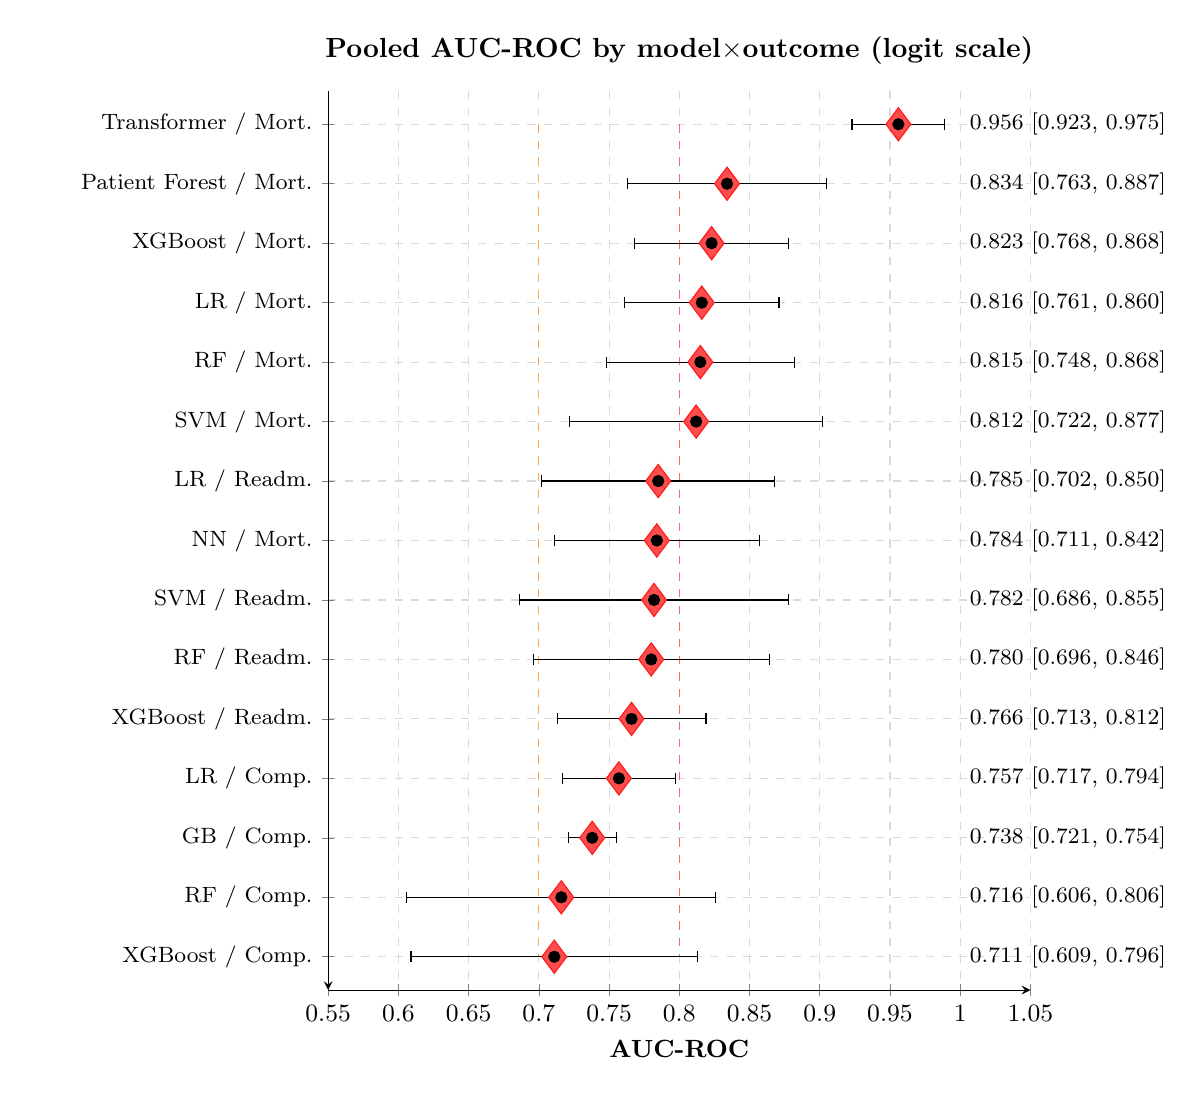
\begin{tikzpicture}
\begin{axis}[
    width=10.5cm, height=13cm,
    symbolic y coords={
        {Transformer / Mort.},
        {Patient Forest / Mort.},
        {XGBoost / Mort.},
        {LR / Mort.},
        {RF / Mort.},
        {SVM / Mort.},
        {LR / Readm.},
        {NN / Mort.},
        {SVM / Readm.},
        {RF / Readm.},
        {XGBoost / Readm.},
        {LR / Comp.},
        {GB / Comp.},
        {RF / Comp.},
        {XGBoost / Comp.}
    },
    ytick=data,
    y dir=reverse,
    xmin=0.55, xmax=1.05,
    xlabel={AUC-ROC}, xlabel style={font=\small\bfseries},
    yticklabel style={font=\footnotesize, text width=3.5cm, align=right},
    xticklabel style={font=\small},
    grid=major, grid style={dashed, gray!30},
    axis lines=left, clip=false, enlarge y limits=0.04,
    title={\textbf{Pooled AUC-ROC by model$\times$outcome (logit scale)}}, title style={font=\normalsize},
]
\draw[red!60, dashed, thin] (axis cs:0.80,{Transformer / Mort.}) -- (axis cs:0.80,{XGBoost / Comp.});
\draw[orange!70, dashed, thin] (axis cs:0.70,{Transformer / Mort.}) -- (axis cs:0.70,{XGBoost / Comp.});
\addplot[only marks, mark=diamond*, mark size=6pt, fill=red!70, draw=red!90]
    coordinates {
(0.956,{Transformer / Mort.})
(0.834,{Patient Forest / Mort.})
(0.823,{XGBoost / Mort.})
(0.816,{LR / Mort.})
(0.815,{RF / Mort.})
(0.812,{SVM / Mort.})
(0.785,{LR / Readm.})
(0.784,{NN / Mort.})
(0.782,{SVM / Readm.})
(0.780,{RF / Readm.})
(0.766,{XGBoost / Readm.})
(0.757,{LR / Comp.})
(0.738,{GB / Comp.})
(0.716,{RF / Comp.})
(0.711,{XGBoost / Comp.})
    };
\addplot[only marks, mark=none, forget plot,
    error bars/.cd, x dir=both, x explicit, error bar style={thin, black}]
    coordinates {
(0.956,{Transformer / Mort.}) +- (0.0330,0.0190)
(0.834,{Patient Forest / Mort.}) +- (0.0710,0.0530)
(0.823,{XGBoost / Mort.}) +- (0.0550,0.0450)
(0.816,{LR / Mort.}) +- (0.0550,0.0440)
(0.815,{RF / Mort.}) +- (0.0670,0.0530)
(0.812,{SVM / Mort.}) +- (0.0900,0.0650)
(0.785,{LR / Readm.}) +- (0.0830,0.0650)
(0.784,{NN / Mort.}) +- (0.0730,0.0580)
(0.782,{SVM / Readm.}) +- (0.0960,0.0730)
(0.780,{RF / Readm.}) +- (0.0840,0.0660)
(0.766,{XGBoost / Readm.}) +- (0.0530,0.0460)
(0.757,{LR / Comp.}) +- (0.0400,0.0370)
(0.738,{GB / Comp.}) +- (0.0170,0.0160)
(0.716,{RF / Comp.}) +- (0.1100,0.0800)
(0.711,{XGBoost / Comp.}) +- (0.1020,0.0850)
    };
\node[anchor=west, font=\footnotesize] at (axis cs:1.00,{Transformer / Mort.}) {0.956 [0.923, 0.975]};
\node[anchor=west, font=\footnotesize] at (axis cs:1.00,{Patient Forest / Mort.}) {0.834 [0.763, 0.887]};
\node[anchor=west, font=\footnotesize] at (axis cs:1.00,{XGBoost / Mort.}) {0.823 [0.768, 0.868]};
\node[anchor=west, font=\footnotesize] at (axis cs:1.00,{LR / Mort.}) {0.816 [0.761, 0.860]};
\node[anchor=west, font=\footnotesize] at (axis cs:1.00,{RF / Mort.}) {0.815 [0.748, 0.868]};
\node[anchor=west, font=\footnotesize] at (axis cs:1.00,{SVM / Mort.}) {0.812 [0.722, 0.877]};
\node[anchor=west, font=\footnotesize] at (axis cs:1.00,{LR / Readm.}) {0.785 [0.702, 0.850]};
\node[anchor=west, font=\footnotesize] at (axis cs:1.00,{NN / Mort.}) {0.784 [0.711, 0.842]};
\node[anchor=west, font=\footnotesize] at (axis cs:1.00,{SVM / Readm.}) {0.782 [0.686, 0.855]};
\node[anchor=west, font=\footnotesize] at (axis cs:1.00,{RF / Readm.}) {0.780 [0.696, 0.846]};
\node[anchor=west, font=\footnotesize] at (axis cs:1.00,{XGBoost / Readm.}) {0.766 [0.713, 0.812]};
\node[anchor=west, font=\footnotesize] at (axis cs:1.00,{LR / Comp.}) {0.757 [0.717, 0.794]};
\node[anchor=west, font=\footnotesize] at (axis cs:1.00,{GB / Comp.}) {0.738 [0.721, 0.754]};
\node[anchor=west, font=\footnotesize] at (axis cs:1.00,{RF / Comp.}) {0.716 [0.606, 0.806]};
\node[anchor=west, font=\footnotesize] at (axis cs:1.00,{XGBoost / Comp.}) {0.711 [0.609, 0.796]};
\end{axis}
\end{tikzpicture}
\caption{Global AUC-ROC forest plot: pooled effect by model$\times$outcome stratum
(random-effects, logit-scale pooling with inverse-variance weighting). Only the 15
model$\times$outcome strata with $k\geq2$ contributing estimates are shown, so that no
row pools estimates for different outcomes (mortality, readmission, or composite)
within the same model -- this replaces an earlier version of this figure that grouped
by model only and mixed outcomes in most rows. Reference lines: AUC\,=\,0.70 (orange)
and AUC\,=\,0.80 (red). Sun M. et al. (2024) is excluded from AUC-ROC pooling (see
Section~\ref{sec:se-tier-note} below and the main manuscript, Section~2.10.4) and does
not contribute to any row of this figure; its estimates are reported descriptively in
Table~\ref{tab:detalle_auc}.}
\label{fig:fp_global}
\end{figure}

\begin{landscape}
\section{Individual AUC-ROC Forest Plots by Model}
\label{sec:se-tier-note}

\subsection{Logistic Regression (11 entries, 5 studies), stratified by outcome}

\begin{figure}[H]
\centering
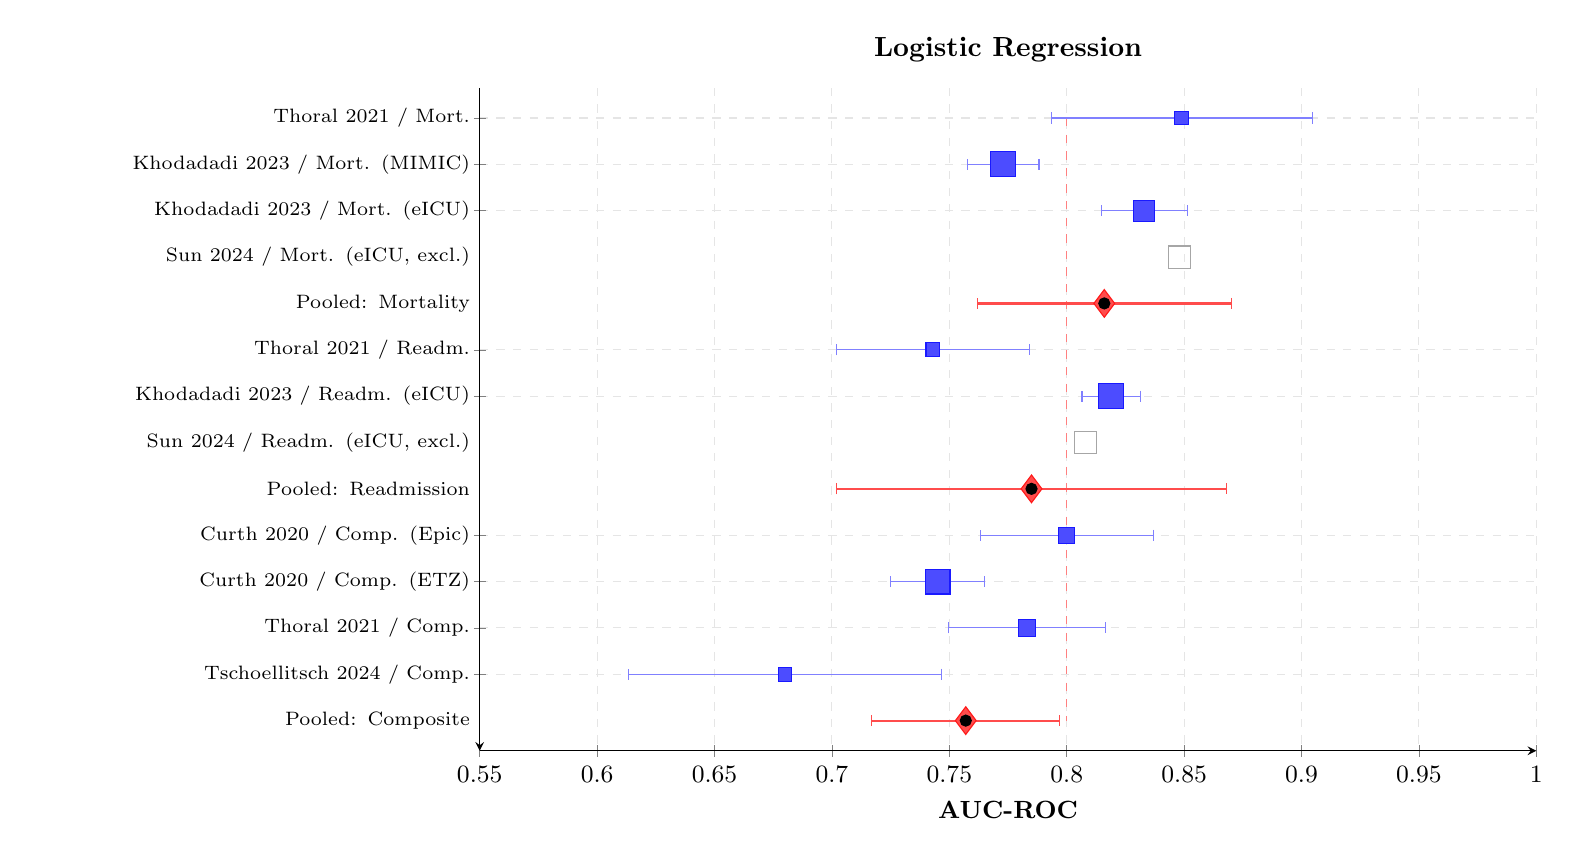
\begin{tikzpicture}[scale=1.0, every node/.style={scale=1.0}]
\begin{axis}[
    width=15cm, height=10cm,
    symbolic y coords={
        {Thoral 2021 / Mort.},
        {Khodadadi 2023 / Mort. (MIMIC)},
        {Khodadadi 2023 / Mort. (eICU)},
        {Sun 2024 / Mort. (eICU, excl.)},
        {Pooled: Mortality},
        {Thoral 2021 / Readm.},
        {Khodadadi 2023 / Readm. (eICU)},
        {Sun 2024 / Readm. (eICU, excl.)},
        {Pooled: Readmission},
        {Curth 2020 / Comp. (Epic)},
        {Curth 2020 / Comp. (ETZ)},
        {Thoral 2021 / Comp.},
        {Tschoellitsch 2024 / Comp.},
        {Pooled: Composite}
    },
    ytick=data,
    y dir=reverse,
    yticklabel=\empty,
    xmin=0.55, xmax=1.00,
    xlabel={AUC-ROC},
    xlabel style={font=\small\bfseries},
    xticklabel style={font=\small},
    grid=major,
    grid style={dashed, gray!20},
    axis lines=left,
    clip=false,
    enlarge y limits=0.05,
    title={\textbf{Logistic Regression}},
    title style={font=\normalsize},
]
\node[anchor=east, font=\scriptsize, text width=5.5cm, align=right] at (axis cs:0.55,{Thoral 2021 / Mort.}) {Thoral 2021 / Mort.};
\node[anchor=east, font=\scriptsize, text width=5.5cm, align=right] at (axis cs:0.55,{Khodadadi 2023 / Mort. (MIMIC)}) {Khodadadi 2023 / Mort. (MIMIC)};
\node[anchor=east, font=\scriptsize, text width=5.5cm, align=right] at (axis cs:0.55,{Khodadadi 2023 / Mort. (eICU)}) {Khodadadi 2023 / Mort. (eICU)};
\node[anchor=east, font=\scriptsize, text width=5.5cm, align=right] at (axis cs:0.55,{Sun 2024 / Mort. (eICU, excl.)}) {Sun 2024 / Mort. (eICU, excl.)};
\node[anchor=east, font=\scriptsize, text width=5.5cm, align=right] at (axis cs:0.55,{Pooled: Mortality}) {Pooled: Mortality};
\node[anchor=east, font=\scriptsize, text width=5.5cm, align=right] at (axis cs:0.55,{Thoral 2021 / Readm.}) {Thoral 2021 / Readm.};
\node[anchor=east, font=\scriptsize, text width=5.5cm, align=right] at (axis cs:0.55,{Khodadadi 2023 / Readm. (eICU)}) {Khodadadi 2023 / Readm. (eICU)};
\node[anchor=east, font=\scriptsize, text width=5.5cm, align=right] at (axis cs:0.55,{Sun 2024 / Readm. (eICU, excl.)}) {Sun 2024 / Readm. (eICU, excl.)};
\node[anchor=east, font=\scriptsize, text width=5.5cm, align=right] at (axis cs:0.55,{Pooled: Readmission}) {Pooled: Readmission};
\node[anchor=east, font=\scriptsize, text width=5.5cm, align=right] at (axis cs:0.55,{Curth 2020 / Comp. (Epic)}) {Curth 2020 / Comp. (Epic)};
\node[anchor=east, font=\scriptsize, text width=5.5cm, align=right] at (axis cs:0.55,{Curth 2020 / Comp. (ETZ)}) {Curth 2020 / Comp. (ETZ)};
\node[anchor=east, font=\scriptsize, text width=5.5cm, align=right] at (axis cs:0.55,{Thoral 2021 / Comp.}) {Thoral 2021 / Comp.};
\node[anchor=east, font=\scriptsize, text width=5.5cm, align=right] at (axis cs:0.55,{Tschoellitsch 2024 / Comp.}) {Tschoellitsch 2024 / Comp.};
\node[anchor=east, font=\scriptsize, text width=5.5cm, align=right] at (axis cs:0.55,{Pooled: Composite}) {Pooled: Composite};

\draw[red!50, dashed, thin] (axis cs:0.80,{Thoral 2021 / Mort.}) -- (axis cs:0.80,{Pooled: Composite});

\addplot[only marks, mark=none,
    error bars/.cd, x dir=both, x explicit, error bar style={thin, blue!50}]
    coordinates {
(0.849,{Thoral 2021 / Mort.}) +- (0.0555,0)
(0.773,{Khodadadi 2023 / Mort. (MIMIC)}) +- (0.0152,0)
(0.833,{Khodadadi 2023 / Mort. (eICU)}) +- (0.0183,0)
(0.743,{Thoral 2021 / Readm.}) +- (0.0410,0)
(0.819,{Khodadadi 2023 / Readm. (eICU)}) +- (0.0125,0)
(0.800,{Curth 2020 / Comp. (Epic)}) +- (0.0368,0)
(0.745,{Curth 2020 / Comp. (ETZ)}) +- (0.0199,0)
(0.783,{Thoral 2021 / Comp.}) +- (0.0335,0)
(0.680,{Tschoellitsch 2024 / Comp.}) +- (0.0665,0)
    };
% Markers with size proportional to each estimate's inverse-variance weight
% within its own model x outcome pooling stratum (weight ~ 1/SE^2)
\addplot[only marks, mark=square*, fill=blue!70, mark size=2.50pt, draw=blue!90] coordinates {(0.849,{Thoral 2021 / Mort.})};
\addplot[only marks, mark=square*, fill=blue!70, mark size=4.50pt, draw=blue!90] coordinates {(0.773,{Khodadadi 2023 / Mort. (MIMIC)})};
\addplot[only marks, mark=square*, fill=blue!70, mark size=3.83pt, draw=blue!90] coordinates {(0.833,{Khodadadi 2023 / Mort. (eICU)})};
\addplot[only marks, mark=square*, fill=blue!70, mark size=2.50pt, draw=blue!90] coordinates {(0.743,{Thoral 2021 / Readm.})};
\addplot[only marks, mark=square*, fill=blue!70, mark size=4.50pt, draw=blue!90] coordinates {(0.819,{Khodadadi 2023 / Readm. (eICU)})};
\addplot[only marks, mark=square*, fill=blue!70, mark size=2.94pt, draw=blue!90] coordinates {(0.800,{Curth 2020 / Comp. (Epic)})};
\addplot[only marks, mark=square*, fill=blue!70, mark size=4.50pt, draw=blue!90] coordinates {(0.745,{Curth 2020 / Comp. (ETZ)})};
\addplot[only marks, mark=square*, fill=blue!70, mark size=3.08pt, draw=blue!90] coordinates {(0.783,{Thoral 2021 / Comp.})};
\addplot[only marks, mark=square*, fill=blue!70, mark size=2.50pt, draw=blue!90] coordinates {(0.680,{Tschoellitsch 2024 / Comp.})};
% Sun M. et al. estimates: excluded from pooling (no event count reported; main text Section 2.10.4)
\addplot[only marks, mark=square, draw=gray!70, mark size=4pt] coordinates {
(0.848,{Sun 2024 / Mort. (eICU, excl.)}) (0.808,{Sun 2024 / Readm. (eICU, excl.)})
};

\addplot[only marks, mark=diamond*, fill=red!70, mark size=5pt, draw=red!90]
    coordinates {(0.816,{Pooled: Mortality}) (0.785,{Pooled: Readmission}) (0.757,{Pooled: Composite})};
\addplot[only marks, mark=none, forget plot,
    error bars/.cd, x dir=both, x explicit, error bar style={thick, red!70}]
    coordinates {
(0.816,{Pooled: Mortality}) +- (0.0541,0.0441)
(0.785,{Pooled: Readmission}) +- (0.0830,0.0648)
(0.757,{Pooled: Composite}) +- (0.0400,0.0368)
    };

\end{axis}
\end{tikzpicture}
\caption{Forest plot --- Logistic Regression, stratified by outcome (main text,
Section~2.10.4). Pooled effects: Mortality 0.816 (95\% CI: 0.761--0.860); Readmission
0.785 (95\% CI: 0.702--0.850); Composite 0.757 (95\% CI: 0.717--0.794). Sun M. et al.~\cite{Sun2024} estimates (hollow markers) are excluded from pooling but shown
descriptively. Previously reported as a single pooled value (0.790) mixing all three
outcomes.}
\label{fig:fp_lr}
\end{figure}
\end{landscape}

\newpage

\begin{landscape}
\subsection{Random Forest (10 entries, 4 studies), stratified by outcome}

\begin{figure}[H]
\centering
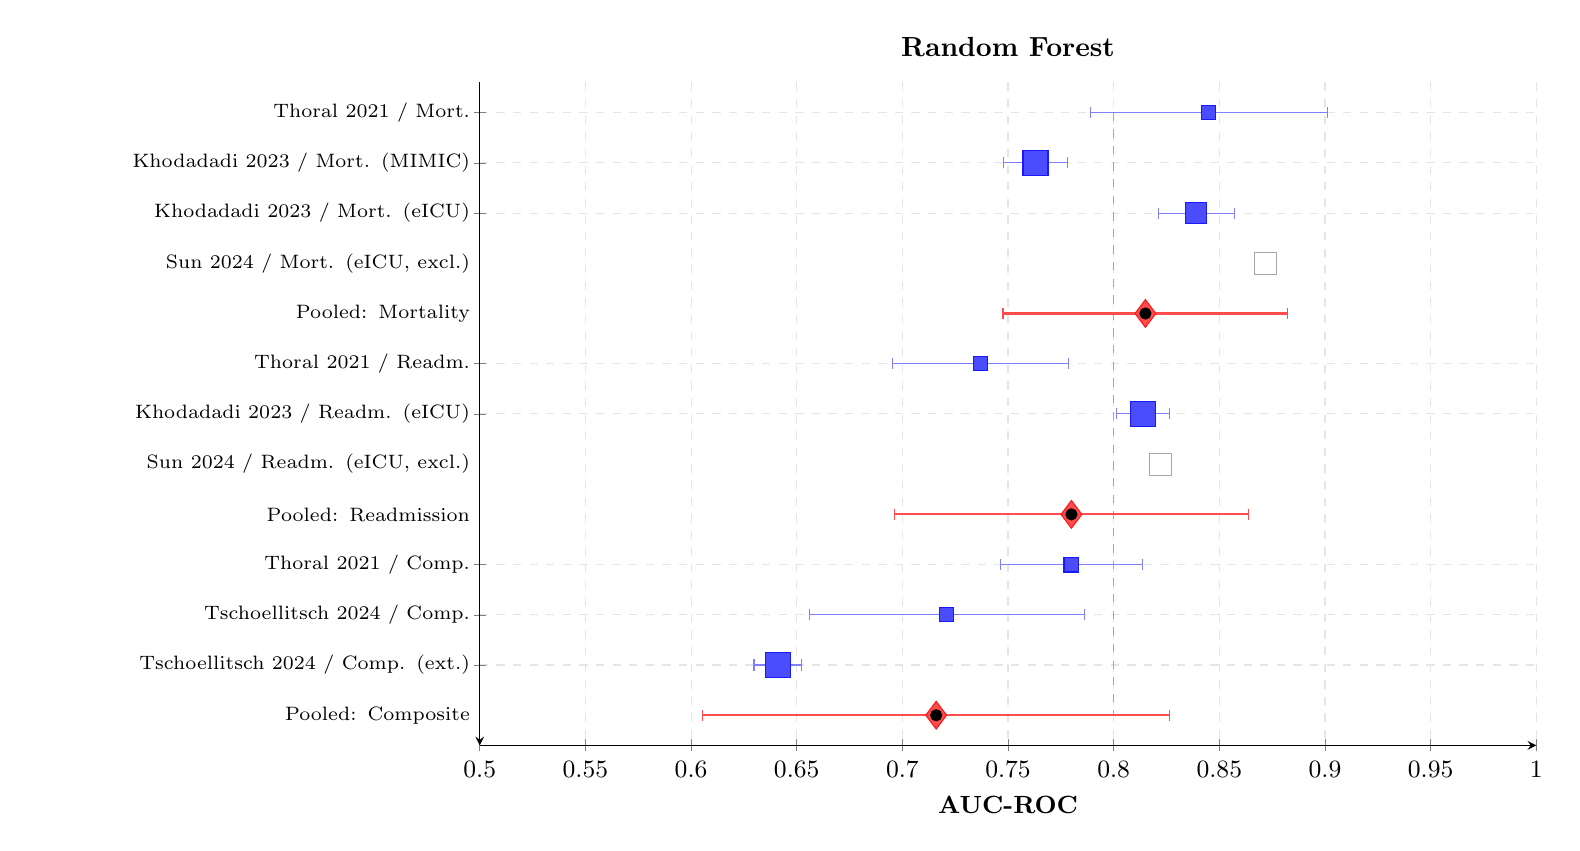
\begin{tikzpicture}[scale=1.0, every node/.style={scale=1.0}]
\begin{axis}[
    width=15cm, height=10cm,
    symbolic y coords={
        {Thoral 2021 / Mort.},
        {Khodadadi 2023 / Mort. (MIMIC)},
        {Khodadadi 2023 / Mort. (eICU)},
        {Sun 2024 / Mort. (eICU, excl.)},
        {Pooled: Mortality},
        {Thoral 2021 / Readm.},
        {Khodadadi 2023 / Readm. (eICU)},
        {Sun 2024 / Readm. (eICU, excl.)},
        {Pooled: Readmission},
        {Thoral 2021 / Comp.},
        {Tschoellitsch 2024 / Comp.},
        {Tschoellitsch 2024 / Comp. (ext.)},
        {Pooled: Composite}
    },
    ytick=data,
    y dir=reverse,
    yticklabel=\empty,
    xmin=0.50, xmax=1.00,
    xlabel={AUC-ROC},
    xlabel style={font=\small\bfseries},
    xticklabel style={font=\small},
    grid=major,
    grid style={dashed, gray!20},
    axis lines=left,
    clip=false,
    enlarge y limits=0.05,
    title={\textbf{Random Forest}},
    title style={font=\normalsize},
]
\node[anchor=east, font=\scriptsize, text width=5.5cm, align=right] at (axis cs:0.50,{Thoral 2021 / Mort.}) {Thoral 2021 / Mort.};
\node[anchor=east, font=\scriptsize, text width=5.5cm, align=right] at (axis cs:0.50,{Khodadadi 2023 / Mort. (MIMIC)}) {Khodadadi 2023 / Mort. (MIMIC)};
\node[anchor=east, font=\scriptsize, text width=5.5cm, align=right] at (axis cs:0.50,{Khodadadi 2023 / Mort. (eICU)}) {Khodadadi 2023 / Mort. (eICU)};
\node[anchor=east, font=\scriptsize, text width=5.5cm, align=right] at (axis cs:0.50,{Sun 2024 / Mort. (eICU, excl.)}) {Sun 2024 / Mort. (eICU, excl.)};
\node[anchor=east, font=\scriptsize, text width=5.5cm, align=right] at (axis cs:0.50,{Pooled: Mortality}) {Pooled: Mortality};
\node[anchor=east, font=\scriptsize, text width=5.5cm, align=right] at (axis cs:0.50,{Thoral 2021 / Readm.}) {Thoral 2021 / Readm.};
\node[anchor=east, font=\scriptsize, text width=5.5cm, align=right] at (axis cs:0.50,{Khodadadi 2023 / Readm. (eICU)}) {Khodadadi 2023 / Readm. (eICU)};
\node[anchor=east, font=\scriptsize, text width=5.5cm, align=right] at (axis cs:0.50,{Sun 2024 / Readm. (eICU, excl.)}) {Sun 2024 / Readm. (eICU, excl.)};
\node[anchor=east, font=\scriptsize, text width=5.5cm, align=right] at (axis cs:0.50,{Pooled: Readmission}) {Pooled: Readmission};
\node[anchor=east, font=\scriptsize, text width=5.5cm, align=right] at (axis cs:0.50,{Thoral 2021 / Comp.}) {Thoral 2021 / Comp.};
\node[anchor=east, font=\scriptsize, text width=5.5cm, align=right] at (axis cs:0.50,{Tschoellitsch 2024 / Comp.}) {Tschoellitsch 2024 / Comp.};
\node[anchor=east, font=\scriptsize, text width=5.5cm, align=right] at (axis cs:0.50,{Tschoellitsch 2024 / Comp. (ext.)}) {Tschoellitsch 2024 / Comp. (ext.)};
\node[anchor=east, font=\scriptsize, text width=5.5cm, align=right] at (axis cs:0.50,{Pooled: Composite}) {Pooled: Composite};

\draw[red!50, dashed, thin] (axis cs:0.80,{Thoral 2021 / Mort.}) -- (axis cs:0.80,{Pooled: Composite});

\addplot[only marks, mark=none,
    error bars/.cd, x dir=both, x explicit, error bar style={thin, blue!50}]
    coordinates {
(0.845,{Thoral 2021 / Mort.}) +- (0.0560,0)
(0.763,{Khodadadi 2023 / Mort. (MIMIC)}) +- (0.0153,0)
(0.839,{Khodadadi 2023 / Mort. (eICU)}) +- (0.0180,0)
(0.737,{Thoral 2021 / Readm.}) +- (0.0415,0)
(0.814,{Khodadadi 2023 / Readm. (eICU)}) +- (0.0126,0)
(0.780,{Thoral 2021 / Comp.}) +- (0.0335,0)
(0.721,{Tschoellitsch 2024 / Comp.}) +- (0.0650,0)
(0.641,{Tschoellitsch 2024 / Comp. (ext.)}) +- (0.0112,0)
    };
% Markers with size proportional to each estimate's inverse-variance weight
% within its own model x outcome pooling stratum (weight ~ 1/SE^2)
\addplot[only marks, mark=square*, fill=blue!70, mark size=2.50pt, draw=blue!90] coordinates {(0.845,{Thoral 2021 / Mort.})};
\addplot[only marks, mark=square*, fill=blue!70, mark size=4.50pt, draw=blue!90] coordinates {(0.763,{Khodadadi 2023 / Mort. (MIMIC)})};
\addplot[only marks, mark=square*, fill=blue!70, mark size=3.90pt, draw=blue!90] coordinates {(0.839,{Khodadadi 2023 / Mort. (eICU)})};
\addplot[only marks, mark=square*, fill=blue!70, mark size=2.50pt, draw=blue!90] coordinates {(0.737,{Thoral 2021 / Readm.})};
\addplot[only marks, mark=square*, fill=blue!70, mark size=4.50pt, draw=blue!90] coordinates {(0.814,{Khodadadi 2023 / Readm. (eICU)})};
\addplot[only marks, mark=square*, fill=blue!70, mark size=2.67pt, draw=blue!90] coordinates {(0.780,{Thoral 2021 / Comp.})};
\addplot[only marks, mark=square*, fill=blue!70, mark size=2.50pt, draw=blue!90] coordinates {(0.721,{Tschoellitsch 2024 / Comp.})};
\addplot[only marks, mark=square*, fill=blue!70, mark size=4.50pt, draw=blue!90] coordinates {(0.641,{Tschoellitsch 2024 / Comp. (ext.)})};
\addplot[only marks, mark=square, draw=gray!70, mark size=4pt] coordinates {
(0.872,{Sun 2024 / Mort. (eICU, excl.)}) (0.822,{Sun 2024 / Readm. (eICU, excl.)})
};

\addplot[only marks, mark=diamond*, fill=red!70, mark size=5pt, draw=red!90]
    coordinates {(0.815,{Pooled: Mortality}) (0.780,{Pooled: Readmission}) (0.716,{Pooled: Composite})};
\addplot[only marks, mark=none, forget plot,
    error bars/.cd, x dir=both, x explicit, error bar style={thick, red!70}]
    coordinates {
(0.815,{Pooled: Mortality}) +- (0.0674,0.0526)
(0.780,{Pooled: Readmission}) +- (0.0838,0.0658)
(0.716,{Pooled: Composite}) +- (0.1105,0.0895)
    };

\end{axis}
\end{tikzpicture}
\caption{Forest plot --- Random Forest, stratified by outcome. Pooled effects: Mortality
0.815 (95\% CI: 0.748--0.868); Readmission 0.780 (95\% CI: 0.696--0.846); Composite 0.716
(95\% CI: 0.606--0.806). Sun M. et al.~\cite{Sun2024} estimates (hollow markers) are
excluded from pooling but shown descriptively. Previously reported as a single pooled
value (0.783) mixing all three outcomes.}
\label{fig:fp_rf}
\end{figure}
\end{landscape}

\newpage

\begin{landscape}
\subsection{XGBoost (10 entries, 4 studies), stratified by outcome}

\begin{figure}[H]
\centering
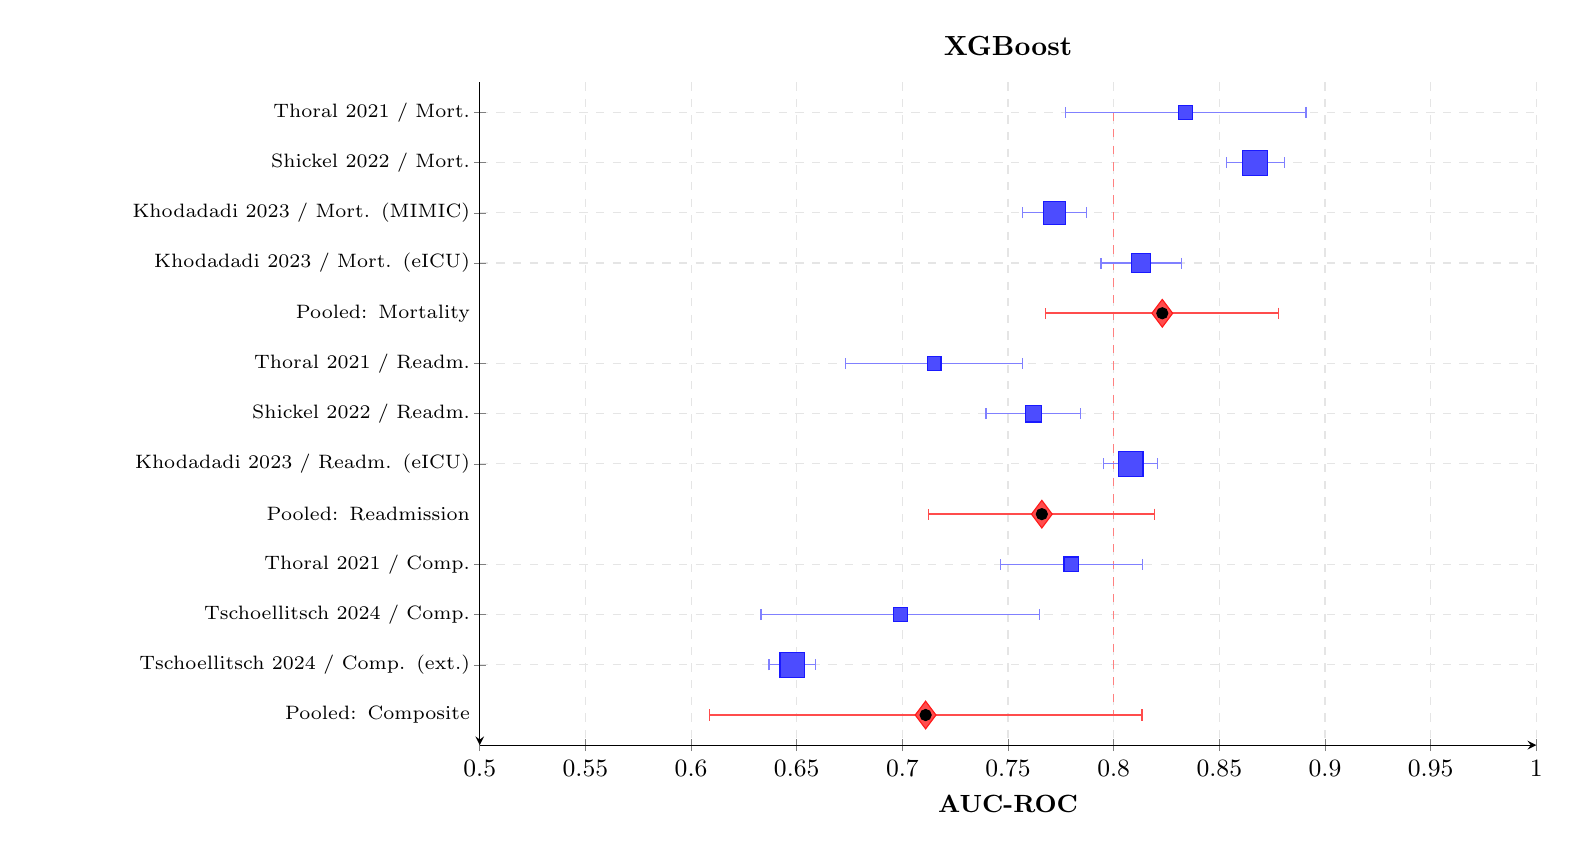
\begin{tikzpicture}[scale=1.0, every node/.style={scale=1.0}]
\begin{axis}[
    width=15cm, height=10cm,
    symbolic y coords={
        {Thoral 2021 / Mort.},
        {Shickel 2022 / Mort.},
        {Khodadadi 2023 / Mort. (MIMIC)},
        {Khodadadi 2023 / Mort. (eICU)},
        {Pooled: Mortality},
        {Thoral 2021 / Readm.},
        {Shickel 2022 / Readm.},
        {Khodadadi 2023 / Readm. (eICU)},
        {Pooled: Readmission},
        {Thoral 2021 / Comp.},
        {Tschoellitsch 2024 / Comp.},
        {Tschoellitsch 2024 / Comp. (ext.)},
        {Pooled: Composite}
    },
    ytick=data,
    y dir=reverse,
    yticklabel=\empty,
    xmin=0.50, xmax=1.00,
    xlabel={AUC-ROC},
    xlabel style={font=\small\bfseries},
    xticklabel style={font=\small},
    grid=major,
    grid style={dashed, gray!20},
    axis lines=left,
    clip=false,
    enlarge y limits=0.05,
    title={\textbf{XGBoost}},
    title style={font=\normalsize},
]
\node[anchor=east, font=\scriptsize, text width=5.5cm, align=right] at (axis cs:0.50,{Thoral 2021 / Mort.}) {Thoral 2021 / Mort.};
\node[anchor=east, font=\scriptsize, text width=5.5cm, align=right] at (axis cs:0.50,{Shickel 2022 / Mort.}) {Shickel 2022 / Mort.};
\node[anchor=east, font=\scriptsize, text width=5.5cm, align=right] at (axis cs:0.50,{Khodadadi 2023 / Mort. (MIMIC)}) {Khodadadi 2023 / Mort. (MIMIC)};
\node[anchor=east, font=\scriptsize, text width=5.5cm, align=right] at (axis cs:0.50,{Khodadadi 2023 / Mort. (eICU)}) {Khodadadi 2023 / Mort. (eICU)};
\node[anchor=east, font=\scriptsize, text width=5.5cm, align=right] at (axis cs:0.50,{Pooled: Mortality}) {Pooled: Mortality};
\node[anchor=east, font=\scriptsize, text width=5.5cm, align=right] at (axis cs:0.50,{Thoral 2021 / Readm.}) {Thoral 2021 / Readm.};
\node[anchor=east, font=\scriptsize, text width=5.5cm, align=right] at (axis cs:0.50,{Shickel 2022 / Readm.}) {Shickel 2022 / Readm.};
\node[anchor=east, font=\scriptsize, text width=5.5cm, align=right] at (axis cs:0.50,{Khodadadi 2023 / Readm. (eICU)}) {Khodadadi 2023 / Readm. (eICU)};
\node[anchor=east, font=\scriptsize, text width=5.5cm, align=right] at (axis cs:0.50,{Pooled: Readmission}) {Pooled: Readmission};
\node[anchor=east, font=\scriptsize, text width=5.5cm, align=right] at (axis cs:0.50,{Thoral 2021 / Comp.}) {Thoral 2021 / Comp.};
\node[anchor=east, font=\scriptsize, text width=5.5cm, align=right] at (axis cs:0.50,{Tschoellitsch 2024 / Comp.}) {Tschoellitsch 2024 / Comp.};
\node[anchor=east, font=\scriptsize, text width=5.5cm, align=right] at (axis cs:0.50,{Tschoellitsch 2024 / Comp. (ext.)}) {Tschoellitsch 2024 / Comp. (ext.)};
\node[anchor=east, font=\scriptsize, text width=5.5cm, align=right] at (axis cs:0.50,{Pooled: Composite}) {Pooled: Composite};

\draw[red!50, dashed, thin] (axis cs:0.80,{Thoral 2021 / Mort.}) -- (axis cs:0.80,{Pooled: Composite});

\addplot[only marks, mark=none,
    error bars/.cd, x dir=both, x explicit, error bar style={thin, blue!50}]
    coordinates {
(0.834,{Thoral 2021 / Mort.}) +- (0.0570,0)
(0.867,{Shickel 2022 / Mort.}) +- (0.0137,0)
(0.772,{Khodadadi 2023 / Mort. (MIMIC)}) +- (0.0152,0)
(0.813,{Khodadadi 2023 / Mort. (eICU)}) +- (0.0190,0)
(0.715,{Thoral 2021 / Readm.}) +- (0.0420,0)
(0.762,{Shickel 2022 / Readm.}) +- (0.0224,0)
(0.808,{Khodadadi 2023 / Readm. (eICU)}) +- (0.0127,0)
(0.780,{Thoral 2021 / Comp.}) +- (0.0335,0)
(0.699,{Tschoellitsch 2024 / Comp.}) +- (0.0659,0)
(0.648,{Tschoellitsch 2024 / Comp. (ext.)}) +- (0.0111,0)
    };
% Markers with size proportional to each estimate's inverse-variance weight
% within its own model x outcome pooling stratum (weight ~ 1/SE^2)
\addplot[only marks, mark=square*, fill=blue!70, mark size=2.50pt, draw=blue!90] coordinates {(0.834,{Thoral 2021 / Mort.})};
\addplot[only marks, mark=square*, fill=blue!70, mark size=4.50pt, draw=blue!90] coordinates {(0.867,{Shickel 2022 / Mort.})};
\addplot[only marks, mark=square*, fill=blue!70, mark size=4.10pt, draw=blue!90] coordinates {(0.772,{Khodadadi 2023 / Mort. (MIMIC)})};
\addplot[only marks, mark=square*, fill=blue!70, mark size=3.48pt, draw=blue!90] coordinates {(0.813,{Khodadadi 2023 / Mort. (eICU)})};
\addplot[only marks, mark=square*, fill=blue!70, mark size=2.50pt, draw=blue!90] coordinates {(0.715,{Thoral 2021 / Readm.})};
\addplot[only marks, mark=square*, fill=blue!70, mark size=3.01pt, draw=blue!90] coordinates {(0.762,{Shickel 2022 / Readm.})};
\addplot[only marks, mark=square*, fill=blue!70, mark size=4.50pt, draw=blue!90] coordinates {(0.808,{Khodadadi 2023 / Readm. (eICU)})};
\addplot[only marks, mark=square*, fill=blue!70, mark size=2.67pt, draw=blue!90] coordinates {(0.780,{Thoral 2021 / Comp.})};
\addplot[only marks, mark=square*, fill=blue!70, mark size=2.50pt, draw=blue!90] coordinates {(0.699,{Tschoellitsch 2024 / Comp.})};
\addplot[only marks, mark=square*, fill=blue!70, mark size=4.50pt, draw=blue!90] coordinates {(0.648,{Tschoellitsch 2024 / Comp. (ext.)})};

\addplot[only marks, mark=diamond*, fill=red!70, mark size=5pt, draw=red!90]
    coordinates {(0.823,{Pooled: Mortality}) (0.766,{Pooled: Readmission}) (0.711,{Pooled: Composite})};
\addplot[only marks, mark=none, forget plot,
    error bars/.cd, x dir=both, x explicit, error bar style={thick, red!70}]
    coordinates {
(0.823,{Pooled: Mortality}) +- (0.0552,0.0443)
(0.766,{Pooled: Readmission}) +- (0.0535,0.0462)
(0.711,{Pooled: Composite}) +- (0.1024,0.0846)
    };

\end{axis}
\end{tikzpicture}
\caption{Forest plot --- XGBoost, stratified by outcome. Pooled effects: Mortality 0.823
(95\% CI: 0.768--0.868); Readmission 0.766 (95\% CI: 0.713--0.812); Composite 0.711 (95\%
CI: 0.609--0.796). Previously reported as a single pooled value (0.770) mixing all three
outcomes.}
\label{fig:fp_xgb}
\end{figure}
\end{landscape}

\newpage

\begin{landscape}
\subsection{Gradient Boosting (9 entries, 3 studies)}

\begin{figure}[H]
\centering
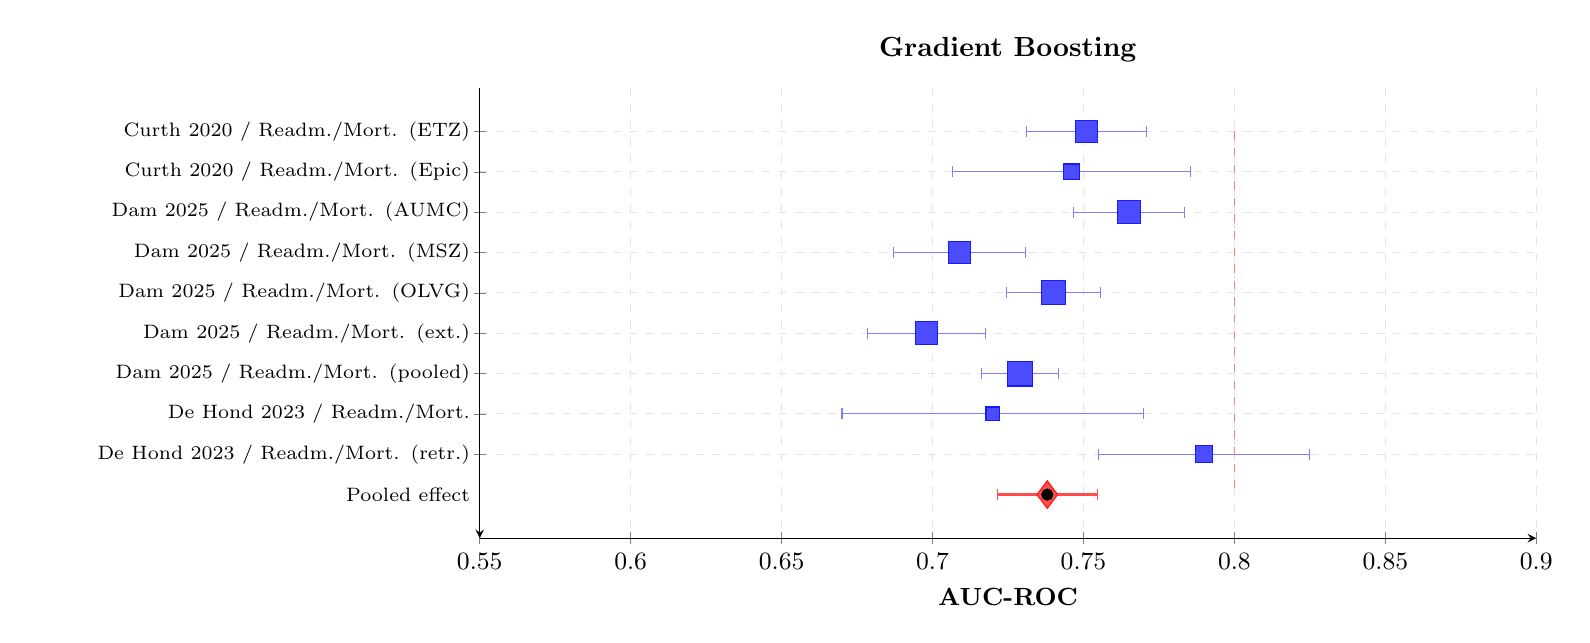
\begin{tikzpicture}[scale=1.0, every node/.style={scale=1.0}]
\begin{axis}[
    width=15cm, height=7.3cm,
    symbolic y coords={
        {Curth 2020 / Readm./Mort. (ETZ)},
        {Curth 2020 / Readm./Mort. (Epic)},
        {Dam 2025 / Readm./Mort. (AUMC)},
        {Dam 2025 / Readm./Mort. (MSZ)},
        {Dam 2025 / Readm./Mort. (OLVG)},
        {Dam 2025 / Readm./Mort. (ext.)},
        {Dam 2025 / Readm./Mort. (pooled)},
        {De Hond 2023 / Readm./Mort.},
        {De Hond 2023 / Readm./Mort. (retr.)},
        Pooled effect
    },
    ytick=data,
    y dir=reverse,
    yticklabel=\empty,
    xmin=0.55, xmax=0.90,
    xlabel={AUC-ROC},
    xlabel style={font=\small\bfseries},
    xticklabel style={font=\small},
    grid=major,
    grid style={dashed, gray!20},
    axis lines=left,
    clip=false,
    enlarge y limits=0.12,
    title={\textbf{Gradient Boosting}},
    title style={font=\normalsize},
]
\node[anchor=east, font=\scriptsize, text width=5.5cm, align=right] at (axis cs:0.55,{Curth 2020 / Readm./Mort. (ETZ)}) {Curth 2020 / Readm./Mort. (ETZ)};
\node[anchor=east, font=\scriptsize, text width=5.5cm, align=right] at (axis cs:0.55,{Curth 2020 / Readm./Mort. (Epic)}) {Curth 2020 / Readm./Mort. (Epic)};
\node[anchor=east, font=\scriptsize, text width=5.5cm, align=right] at (axis cs:0.55,{Dam 2025 / Readm./Mort. (AUMC)}) {Dam 2025 / Readm./Mort. (AUMC)};
\node[anchor=east, font=\scriptsize, text width=5.5cm, align=right] at (axis cs:0.55,{Dam 2025 / Readm./Mort. (MSZ)}) {Dam 2025 / Readm./Mort. (MSZ)};
\node[anchor=east, font=\scriptsize, text width=5.5cm, align=right] at (axis cs:0.55,{Dam 2025 / Readm./Mort. (OLVG)}) {Dam 2025 / Readm./Mort. (OLVG)};
\node[anchor=east, font=\scriptsize, text width=5.5cm, align=right] at (axis cs:0.55,{Dam 2025 / Readm./Mort. (ext.)}) {Dam 2025 / Readm./Mort. (ext.)};
\node[anchor=east, font=\scriptsize, text width=5.5cm, align=right] at (axis cs:0.55,{Dam 2025 / Readm./Mort. (pooled)}) {Dam 2025 / Readm./Mort. (pooled)};
\node[anchor=east, font=\scriptsize, text width=5.5cm, align=right] at (axis cs:0.55,{De Hond 2023 / Readm./Mort.}) {De Hond 2023 / Readm./Mort.};
\node[anchor=east, font=\scriptsize, text width=5.5cm, align=right] at (axis cs:0.55,{De Hond 2023 / Readm./Mort. (retr.)}) {De Hond 2023 / Readm./Mort. (retr.)};
\node[anchor=east, font=\scriptsize, text width=5.5cm, align=right] at (axis cs:0.55,Pooled effect) {Pooled effect};

\draw[red!50, dashed, thin] (axis cs:0.80,{Curth 2020 / Readm./Mort. (ETZ)}) -- (axis cs:0.80,Pooled effect);

\addplot[only marks, mark=none,
    error bars/.cd, x dir=both, x explicit, error bar style={thin, blue!50}]
    coordinates {
(0.751,{Curth 2020 / Readm./Mort. (ETZ)}) +- (0.0198,0)
(0.746,{Curth 2020 / Readm./Mort. (Epic)}) +- (0.0394,0)
(0.765,{Dam 2025 / Readm./Mort. (AUMC)}) +- (0.0184,0)
(0.709,{Dam 2025 / Readm./Mort. (MSZ)}) +- (0.0219,0)
(0.740,{Dam 2025 / Readm./Mort. (OLVG)}) +- (0.0156,0)
(0.698,{Dam 2025 / Readm./Mort. (ext.)}) +- (0.0195,0)
(0.729,{Dam 2025 / Readm./Mort. (pooled)}) +- (0.0127,0)
(0.720,{De Hond 2023 / Readm./Mort.}) +- (0.0500,0.0400)
(0.790,{De Hond 2023 / Readm./Mort. (retr.)}) +- (0.0350,0)
    };
% Markers with size proportional to study weight
\addplot[only marks, mark=square*, fill=blue!70, mark size=4.08pt, draw=blue!90] coordinates {(0.751,{Curth 2020 / Readm./Mort. (ETZ)})};
\addplot[only marks, mark=square*, fill=blue!70, mark size=2.80pt, draw=blue!90] coordinates {(0.746,{Curth 2020 / Readm./Mort. (Epic)})};
\addplot[only marks, mark=square*, fill=blue!70, mark size=4.17pt, draw=blue!90] coordinates {(0.765,{Dam 2025 / Readm./Mort. (AUMC)})};
\addplot[only marks, mark=square*, fill=blue!70, mark size=3.92pt, draw=blue!90] coordinates {(0.709,{Dam 2025 / Readm./Mort. (MSZ)})};
\addplot[only marks, mark=square*, fill=blue!70, mark size=4.32pt, draw=blue!90] coordinates {(0.740,{Dam 2025 / Readm./Mort. (OLVG)})};
\addplot[only marks, mark=square*, fill=blue!70, mark size=4.08pt, draw=blue!90] coordinates {(0.698,{Dam 2025 / Readm./Mort. (ext.)})};
\addplot[only marks, mark=square*, fill=blue!70, mark size=4.50pt, draw=blue!90] coordinates {(0.729,{Dam 2025 / Readm./Mort. (pooled)})};
\addplot[only marks, mark=square*, fill=blue!70, mark size=2.50pt, draw=blue!90] coordinates {(0.720,{De Hond 2023 / Readm./Mort.})};
\addplot[only marks, mark=square*, fill=blue!70, mark size=3.08pt, draw=blue!90] coordinates {(0.790,{De Hond 2023 / Readm./Mort. (retr.)})};

\addplot[only marks, mark=diamond*, fill=red!70, mark size=5pt, draw=red!90]
    coordinates {(0.738,{Pooled effect})};
\addplot[only marks, mark=none, forget plot,
    error bars/.cd, x dir=both, x explicit, error bar style={thick, red!70}]
    coordinates {(0.738,{Pooled effect}) +- (0.0165,0)};

\end{axis}
\end{tikzpicture}
\caption{Forest plot --- Gradient Boosting. Pooled effect: 0.738 (95\% CI: 0.721--0.754).}
\label{fig:fp_gb}
\end{figure}
\end{landscape}

\newpage

\begin{landscape}
\subsection{Transformer (8 entries, 2 studies), stratified by outcome}

\begin{figure}[H]
\centering
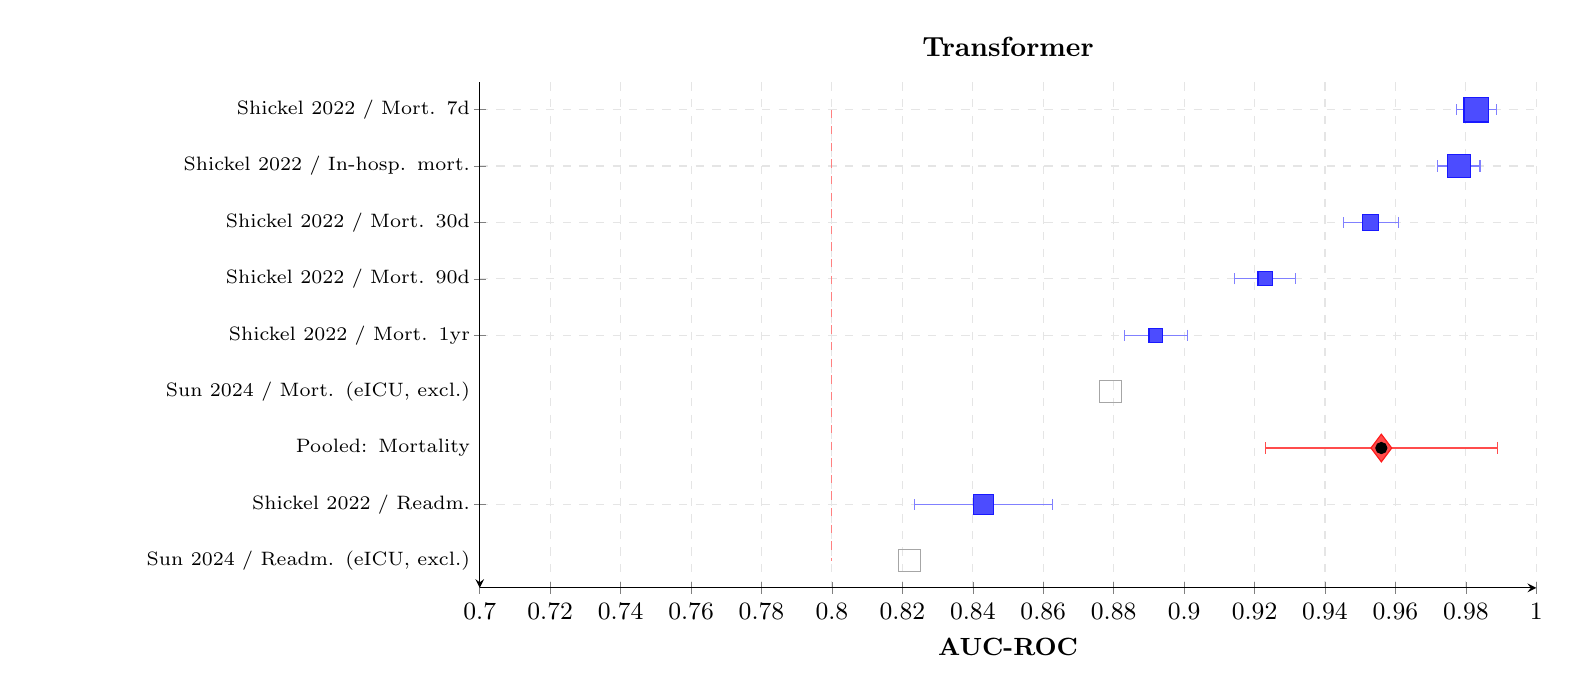
\begin{tikzpicture}[scale=1.0, every node/.style={scale=1.0}]
\begin{axis}[
    width=15cm, height=8cm,
    symbolic y coords={
        {Shickel 2022 / Mort. 7d},
        {Shickel 2022 / In-hosp. mort.},
        {Shickel 2022 / Mort. 30d},
        {Shickel 2022 / Mort. 90d},
        {Shickel 2022 / Mort. 1yr},
        {Sun 2024 / Mort. (eICU, excl.)},
        {Pooled: Mortality},
        {Shickel 2022 / Readm.},
        {Sun 2024 / Readm. (eICU, excl.)}
    },
    ytick=data,
    y dir=reverse,
    yticklabel=\empty,
    xmin=0.70, xmax=1.00,
    xlabel={AUC-ROC},
    xlabel style={font=\small\bfseries},
    xticklabel style={font=\small},
    grid=major,
    grid style={dashed, gray!20},
    axis lines=left,
    clip=false,
    enlarge y limits=0.06,
    title={\textbf{Transformer}},
    title style={font=\normalsize},
]
\node[anchor=east, font=\scriptsize, text width=5.5cm, align=right] at (axis cs:0.70,{Shickel 2022 / Mort. 7d}) {Shickel 2022 / Mort. 7d};
\node[anchor=east, font=\scriptsize, text width=5.5cm, align=right] at (axis cs:0.70,{Shickel 2022 / In-hosp. mort.}) {Shickel 2022 / In-hosp. mort.};
\node[anchor=east, font=\scriptsize, text width=5.5cm, align=right] at (axis cs:0.70,{Shickel 2022 / Mort. 30d}) {Shickel 2022 / Mort. 30d};
\node[anchor=east, font=\scriptsize, text width=5.5cm, align=right] at (axis cs:0.70,{Shickel 2022 / Mort. 90d}) {Shickel 2022 / Mort. 90d};
\node[anchor=east, font=\scriptsize, text width=5.5cm, align=right] at (axis cs:0.70,{Shickel 2022 / Mort. 1yr}) {Shickel 2022 / Mort. 1yr};
\node[anchor=east, font=\scriptsize, text width=5.5cm, align=right] at (axis cs:0.70,{Sun 2024 / Mort. (eICU, excl.)}) {Sun 2024 / Mort. (eICU, excl.)};
\node[anchor=east, font=\scriptsize, text width=5.5cm, align=right] at (axis cs:0.70,{Pooled: Mortality}) {Pooled: Mortality};
\node[anchor=east, font=\scriptsize, text width=5.5cm, align=right] at (axis cs:0.70,{Shickel 2022 / Readm.}) {Shickel 2022 / Readm.};
\node[anchor=east, font=\scriptsize, text width=5.5cm, align=right] at (axis cs:0.70,{Sun 2024 / Readm. (eICU, excl.)}) {Sun 2024 / Readm. (eICU, excl.)};

\draw[red!50, dashed, thin] (axis cs:0.80,{Shickel 2022 / Mort. 7d}) -- (axis cs:0.80,{Sun 2024 / Readm. (eICU, excl.)});

\addplot[only marks, mark=none,
    error bars/.cd, x dir=both, x explicit, error bar style={thin, blue!50}]
    coordinates {
(0.983,{Shickel 2022 / Mort. 7d}) +- (0.0056,0)
(0.978,{Shickel 2022 / In-hosp. mort.}) +- (0.0060,0)
(0.953,{Shickel 2022 / Mort. 30d}) +- (0.0078,0)
(0.923,{Shickel 2022 / Mort. 90d}) +- (0.0087,0)
(0.892,{Shickel 2022 / Mort. 1yr}) +- (0.0089,0)
(0.843,{Shickel 2022 / Readm.}) +- (0.0196,0)
    };
% Markers with size proportional to each estimate's inverse-variance weight
% within its own model x outcome pooling stratum (weight ~ 1/SE^2); the
% readmission estimate is k=1 (not pooled), so it keeps a neutral size
\addplot[only marks, mark=square*, fill=blue!70, mark size=4.50pt, draw=blue!90] coordinates {(0.983,{Shickel 2022 / Mort. 7d})};
\addplot[only marks, mark=square*, fill=blue!70, mark size=4.07pt, draw=blue!90] coordinates {(0.978,{Shickel 2022 / In-hosp. mort.})};
\addplot[only marks, mark=square*, fill=blue!70, mark size=2.90pt, draw=blue!90] coordinates {(0.953,{Shickel 2022 / Mort. 30d})};
\addplot[only marks, mark=square*, fill=blue!70, mark size=2.56pt, draw=blue!90] coordinates {(0.923,{Shickel 2022 / Mort. 90d})};
\addplot[only marks, mark=square*, fill=blue!70, mark size=2.50pt, draw=blue!90] coordinates {(0.892,{Shickel 2022 / Mort. 1yr})};
\addplot[only marks, mark=square*, fill=blue!70, mark size=3.5pt, draw=blue!90] coordinates {(0.843,{Shickel 2022 / Readm.})};
\addplot[only marks, mark=square, draw=gray!70, mark size=4pt] coordinates {
(0.879,{Sun 2024 / Mort. (eICU, excl.)}) (0.822,{Sun 2024 / Readm. (eICU, excl.)})
};

\addplot[only marks, mark=diamond*, fill=red!70, mark size=5pt, draw=red!90]
    coordinates {(0.956,{Pooled: Mortality})};
\addplot[only marks, mark=none, forget plot,
    error bars/.cd, x dir=both, x explicit, error bar style={thick, red!70}]
    coordinates {(0.956,{Pooled: Mortality}) +- (0.0330,0.0190)};

\end{axis}
\end{tikzpicture}
\caption{Forest plot --- Transformer, stratified by outcome. Five mortality estimates
from Shickel et al.~\cite{Shickel2022} at distinct horizons (Table 4, main text) are
pooled: 0.956 (95\% CI: 0.923--0.975; I\textsuperscript{2}=98.5\%). The single
readmission estimate ($k=1$) is not pooled. Sun M. et al.~\cite{Sun2024} estimates (hollow
markers) are excluded from pooling but shown descriptively. Previously reported as a
single pooled value (0.910) mixing mortality and readmission from two studies.}
\label{fig:fp_transformer}
\end{figure}
\end{landscape}

\newpage

\begin{landscape}
\subsection{SVM (6 entries, 2 studies), stratified by outcome}

\begin{figure}[H]
\centering
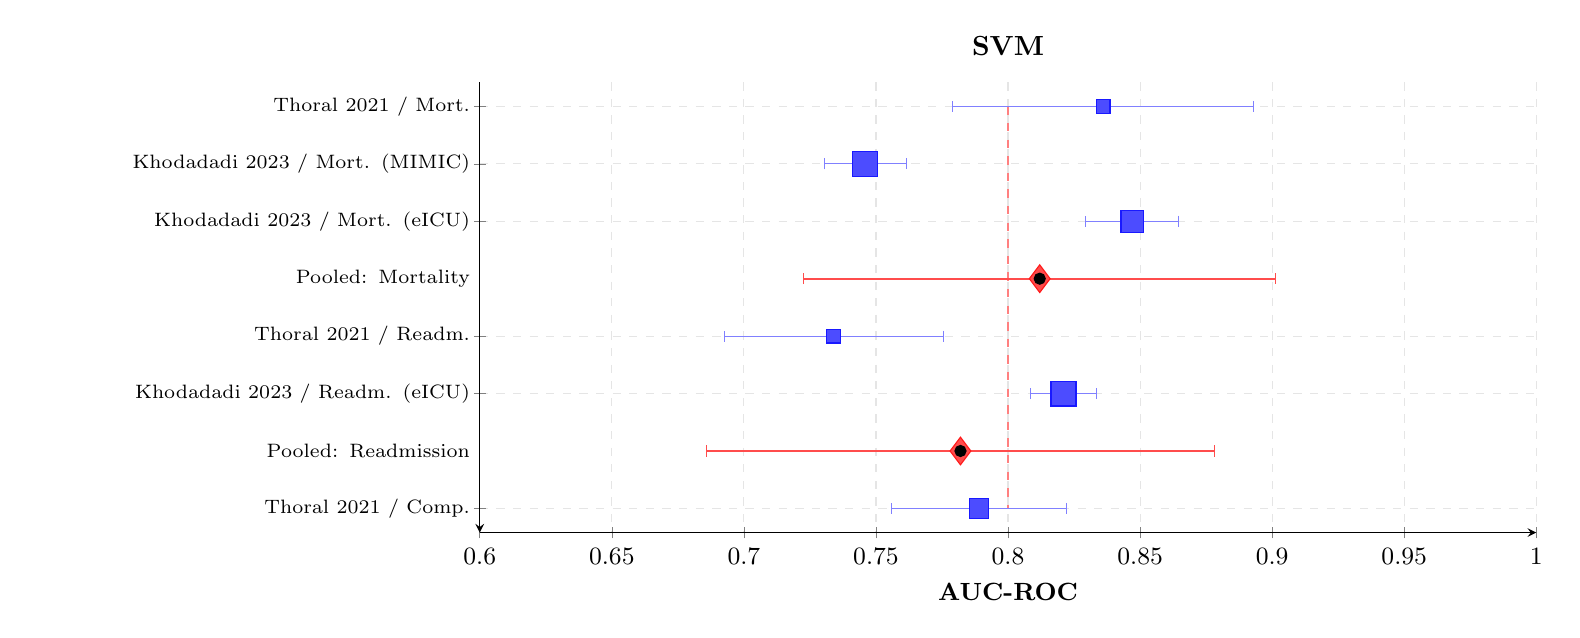
\begin{tikzpicture}[scale=1.0, every node/.style={scale=1.0}]
\begin{axis}[
    width=15cm, height=7.3cm,
    symbolic y coords={
        {Thoral 2021 / Mort.},
        {Khodadadi 2023 / Mort. (MIMIC)},
        {Khodadadi 2023 / Mort. (eICU)},
        {Pooled: Mortality},
        {Thoral 2021 / Readm.},
        {Khodadadi 2023 / Readm. (eICU)},
        {Pooled: Readmission},
        {Thoral 2021 / Comp.}
    },
    ytick=data,
    y dir=reverse,
    yticklabel=\empty,
    xmin=0.60, xmax=1.00,
    xlabel={AUC-ROC},
    xlabel style={font=\small\bfseries},
    xticklabel style={font=\small},
    grid=major,
    grid style={dashed, gray!20},
    axis lines=left,
    clip=false,
    enlarge y limits=0.06,
    title={\textbf{SVM}},
    title style={font=\normalsize},
]
\node[anchor=east, font=\scriptsize, text width=5.5cm, align=right] at (axis cs:0.60,{Thoral 2021 / Mort.}) {Thoral 2021 / Mort.};
\node[anchor=east, font=\scriptsize, text width=5.5cm, align=right] at (axis cs:0.60,{Khodadadi 2023 / Mort. (MIMIC)}) {Khodadadi 2023 / Mort. (MIMIC)};
\node[anchor=east, font=\scriptsize, text width=5.5cm, align=right] at (axis cs:0.60,{Khodadadi 2023 / Mort. (eICU)}) {Khodadadi 2023 / Mort. (eICU)};
\node[anchor=east, font=\scriptsize, text width=5.5cm, align=right] at (axis cs:0.60,{Pooled: Mortality}) {Pooled: Mortality};
\node[anchor=east, font=\scriptsize, text width=5.5cm, align=right] at (axis cs:0.60,{Thoral 2021 / Readm.}) {Thoral 2021 / Readm.};
\node[anchor=east, font=\scriptsize, text width=5.5cm, align=right] at (axis cs:0.60,{Khodadadi 2023 / Readm. (eICU)}) {Khodadadi 2023 / Readm. (eICU)};
\node[anchor=east, font=\scriptsize, text width=5.5cm, align=right] at (axis cs:0.60,{Pooled: Readmission}) {Pooled: Readmission};
\node[anchor=east, font=\scriptsize, text width=5.5cm, align=right] at (axis cs:0.60,{Thoral 2021 / Comp.}) {Thoral 2021 / Comp.};

\draw[red!50, dashed, thin] (axis cs:0.80,{Thoral 2021 / Mort.}) -- (axis cs:0.80,{Thoral 2021 / Comp.});

\addplot[only marks, mark=none,
    error bars/.cd, x dir=both, x explicit, error bar style={thin, blue!50}]
    coordinates {
(0.836,{Thoral 2021 / Mort.}) +- (0.0570,0)
(0.746,{Khodadadi 2023 / Mort. (MIMIC)}) +- (0.0156,0)
(0.847,{Khodadadi 2023 / Mort. (eICU)}) +- (0.0177,0)
(0.734,{Thoral 2021 / Readm.}) +- (0.0415,0)
(0.821,{Khodadadi 2023 / Readm. (eICU)}) +- (0.0124,0)
(0.789,{Thoral 2021 / Comp.}) +- (0.0330,0)
    };
% Markers with size proportional to each estimate's inverse-variance weight
% within its own model x outcome pooling stratum (weight ~ 1/SE^2); the
% composite estimate is k=1 (not pooled), neutral size
\addplot[only marks, mark=square*, fill=blue!70, mark size=2.50pt, draw=blue!90] coordinates {(0.836,{Thoral 2021 / Mort.})};
\addplot[only marks, mark=square*, fill=blue!70, mark size=4.50pt, draw=blue!90] coordinates {(0.746,{Khodadadi 2023 / Mort. (MIMIC)})};
\addplot[only marks, mark=square*, fill=blue!70, mark size=4.02pt, draw=blue!90] coordinates {(0.847,{Khodadadi 2023 / Mort. (eICU)})};
\addplot[only marks, mark=square*, fill=blue!70, mark size=2.50pt, draw=blue!90] coordinates {(0.734,{Thoral 2021 / Readm.})};
\addplot[only marks, mark=square*, fill=blue!70, mark size=4.50pt, draw=blue!90] coordinates {(0.821,{Khodadadi 2023 / Readm. (eICU)})};
\addplot[only marks, mark=square*, fill=blue!70, mark size=3.5pt, draw=blue!90] coordinates {(0.789,{Thoral 2021 / Comp.})};

\addplot[only marks, mark=diamond*, fill=red!70, mark size=5pt, draw=red!90]
    coordinates {(0.812,{Pooled: Mortality}) (0.782,{Pooled: Readmission})};
\addplot[only marks, mark=none, forget plot,
    error bars/.cd, x dir=both, x explicit, error bar style={thick, red!70}]
    coordinates {
(0.812,{Pooled: Mortality}) +- (0.0893,0.0655)
(0.782,{Pooled: Readmission}) +- (0.0963,0.0730)
    };

\end{axis}
\end{tikzpicture}
\caption{Forest plot --- SVM, stratified by outcome. Pooled effects: Mortality 0.812
(95\% CI: 0.722--0.877); Readmission 0.782 (95\% CI: 0.686--0.855). The single composite
estimate ($k=1$) is not pooled. Previously reported as a single pooled value (0.795)
mixing all three outcomes.}
\label{fig:fp_svm}
\end{figure}
\end{landscape}

\begin{landscape}
\subsection{Neural Network (6 entries, 3 studies), stratified by outcome}

\begin{figure}[H]
\centering
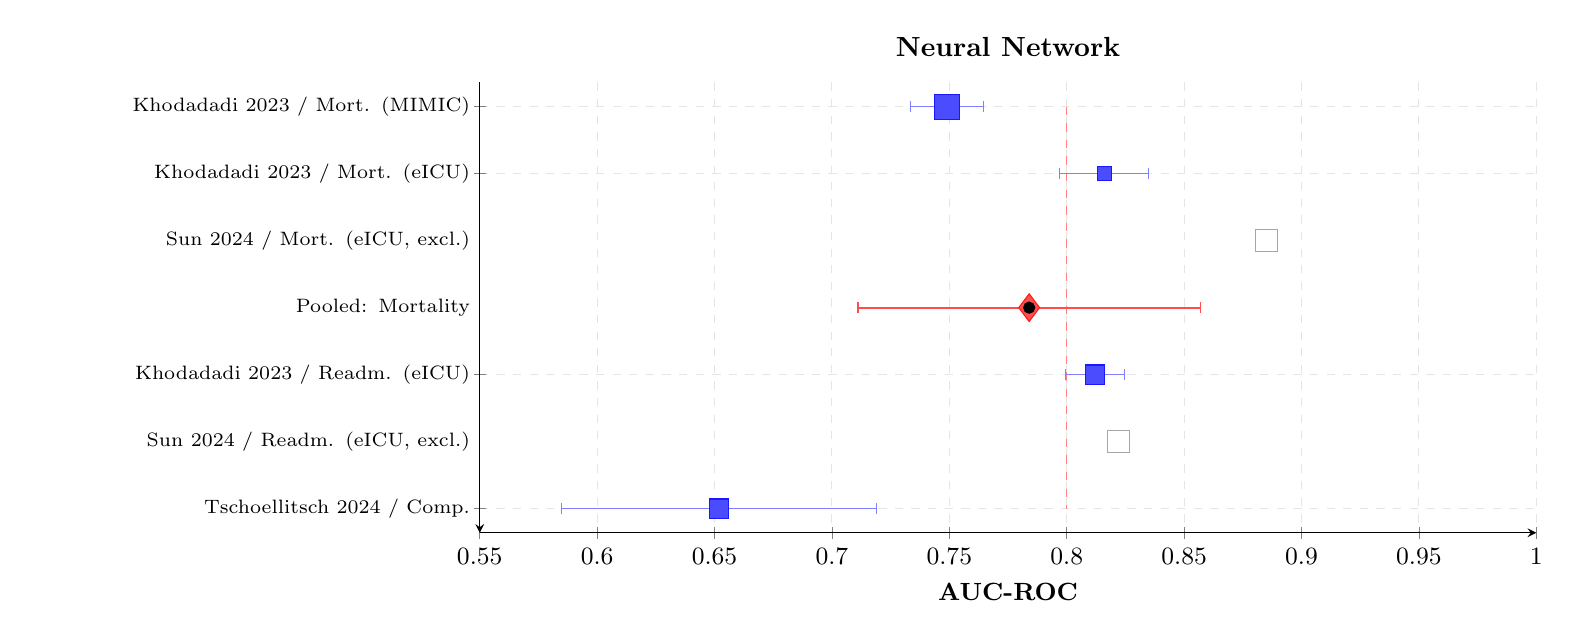
\begin{tikzpicture}[scale=1.0, every node/.style={scale=1.0}]
\begin{axis}[
    width=15cm, height=7.3cm,
    symbolic y coords={
        {Khodadadi 2023 / Mort. (MIMIC)},
        {Khodadadi 2023 / Mort. (eICU)},
        {Sun 2024 / Mort. (eICU, excl.)},
        {Pooled: Mortality},
        {Khodadadi 2023 / Readm. (eICU)},
        {Sun 2024 / Readm. (eICU, excl.)},
        {Tschoellitsch 2024 / Comp.}
    },
    ytick=data,
    y dir=reverse,
    yticklabel=\empty,
    xmin=0.55, xmax=1.00,
    xlabel={AUC-ROC},
    xlabel style={font=\small\bfseries},
    xticklabel style={font=\small},
    grid=major,
    grid style={dashed, gray!20},
    axis lines=left,
    clip=false,
    enlarge y limits=0.06,
    title={\textbf{Neural Network}},
    title style={font=\normalsize},
]
\node[anchor=east, font=\scriptsize, text width=5.5cm, align=right] at (axis cs:0.55,{Khodadadi 2023 / Mort. (MIMIC)}) {Khodadadi 2023 / Mort. (MIMIC)};
\node[anchor=east, font=\scriptsize, text width=5.5cm, align=right] at (axis cs:0.55,{Khodadadi 2023 / Mort. (eICU)}) {Khodadadi 2023 / Mort. (eICU)};
\node[anchor=east, font=\scriptsize, text width=5.5cm, align=right] at (axis cs:0.55,{Sun 2024 / Mort. (eICU, excl.)}) {Sun 2024 / Mort. (eICU, excl.)};
\node[anchor=east, font=\scriptsize, text width=5.5cm, align=right] at (axis cs:0.55,{Pooled: Mortality}) {Pooled: Mortality};
\node[anchor=east, font=\scriptsize, text width=5.5cm, align=right] at (axis cs:0.55,{Khodadadi 2023 / Readm. (eICU)}) {Khodadadi 2023 / Readm. (eICU)};
\node[anchor=east, font=\scriptsize, text width=5.5cm, align=right] at (axis cs:0.55,{Sun 2024 / Readm. (eICU, excl.)}) {Sun 2024 / Readm. (eICU, excl.)};
\node[anchor=east, font=\scriptsize, text width=5.5cm, align=right] at (axis cs:0.55,{Tschoellitsch 2024 / Comp.}) {Tschoellitsch 2024 / Comp.};

\draw[red!50, dashed, thin] (axis cs:0.80,{Khodadadi 2023 / Mort. (MIMIC)}) -- (axis cs:0.80,{Tschoellitsch 2024 / Comp.});

\addplot[only marks, mark=none,
    error bars/.cd, x dir=both, x explicit, error bar style={thin, blue!50}]
    coordinates {
(0.749,{Khodadadi 2023 / Mort. (MIMIC)}) +- (0.0156,0)
(0.816,{Khodadadi 2023 / Mort. (eICU)}) +- (0.0189,0)
(0.812,{Khodadadi 2023 / Readm. (eICU)}) +- (0.0127,0)
(0.652,{Tschoellitsch 2024 / Comp.}) +- (0.0671,0)
    };
% Markers with size proportional to each estimate's inverse-variance weight
% within its own model x outcome pooling stratum (weight ~ 1/SE^2); the
% readmission and composite estimates are k=1 (not pooled), neutral size
\addplot[only marks, mark=square*, fill=blue!70, mark size=4.50pt, draw=blue!90] coordinates {(0.749,{Khodadadi 2023 / Mort. (MIMIC)})};
\addplot[only marks, mark=square*, fill=blue!70, mark size=2.50pt, draw=blue!90] coordinates {(0.816,{Khodadadi 2023 / Mort. (eICU)})};
\addplot[only marks, mark=square*, fill=blue!70, mark size=3.5pt, draw=blue!90] coordinates {(0.812,{Khodadadi 2023 / Readm. (eICU)})};
\addplot[only marks, mark=square*, fill=blue!70, mark size=3.5pt, draw=blue!90] coordinates {(0.652,{Tschoellitsch 2024 / Comp.})};
\addplot[only marks, mark=square, draw=gray!70, mark size=4pt] coordinates {
(0.885,{Sun 2024 / Mort. (eICU, excl.)}) (0.822,{Sun 2024 / Readm. (eICU, excl.)})
};

\addplot[only marks, mark=diamond*, fill=red!70, mark size=5pt, draw=red!90]
    coordinates {(0.784,{Pooled: Mortality})};
\addplot[only marks, mark=none, forget plot,
    error bars/.cd, x dir=both, x explicit, error bar style={thick, red!70}]
    coordinates {(0.784,{Pooled: Mortality}) +- (0.0729,0.0586)};

\end{axis}
\end{tikzpicture}
\caption{Forest plot --- Neural Network, stratified by outcome. Pooled mortality effect:
0.784 (95\% CI: 0.711--0.842). The single readmission and single composite estimates
($k=1$ each) are not pooled. Sun M. et al.~\cite{Sun2024} estimates (hollow markers) are
excluded from pooling but shown descriptively. Previously reported as a single pooled
value (0.791) mixing all three outcomes.}
\label{fig:fp_nn}
\end{figure}
\end{landscape}

\newpage

\begin{landscape}
\subsection{Patient Forest (3 entries, 1 study), stratified by outcome}

\begin{figure}[H]
\centering
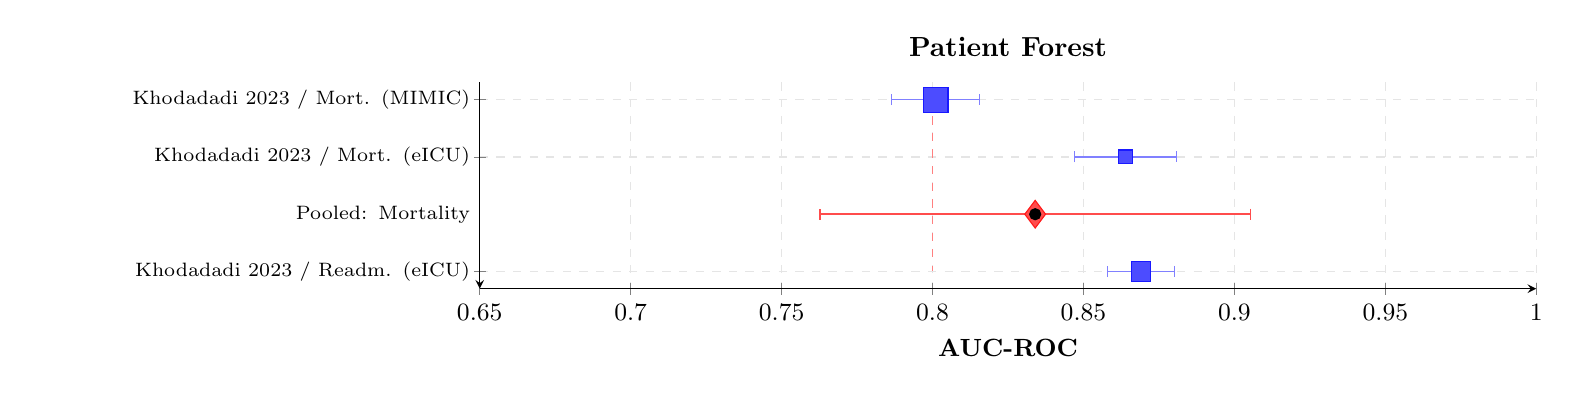
\begin{tikzpicture}[scale=1.0, every node/.style={scale=1.0}]
\begin{axis}[
    width=15cm, height=4.2cm,
    symbolic y coords={
        {Khodadadi 2023 / Mort. (MIMIC)},
        {Khodadadi 2023 / Mort. (eICU)},
        {Pooled: Mortality},
        {Khodadadi 2023 / Readm. (eICU)}
    },
    ytick=data,
    y dir=reverse,
    yticklabel=\empty,
    xmin=0.65, xmax=1.00,
    xlabel={AUC-ROC},
    xlabel style={font=\small\bfseries},
    xticklabel style={font=\small},
    grid=major,
    grid style={dashed, gray!20},
    axis lines=left,
    clip=false,
    enlarge y limits=0.10,
    title={\textbf{Patient Forest}},
    title style={font=\normalsize},
]
\node[anchor=east, font=\scriptsize, text width=5.5cm, align=right] at (axis cs:0.65,{Khodadadi 2023 / Mort. (MIMIC)}) {Khodadadi 2023 / Mort. (MIMIC)};
\node[anchor=east, font=\scriptsize, text width=5.5cm, align=right] at (axis cs:0.65,{Khodadadi 2023 / Mort. (eICU)}) {Khodadadi 2023 / Mort. (eICU)};
\node[anchor=east, font=\scriptsize, text width=5.5cm, align=right] at (axis cs:0.65,{Pooled: Mortality}) {Pooled: Mortality};
\node[anchor=east, font=\scriptsize, text width=5.5cm, align=right] at (axis cs:0.65,{Khodadadi 2023 / Readm. (eICU)}) {Khodadadi 2023 / Readm. (eICU)};

\draw[red!50, dashed, thin] (axis cs:0.80,{Khodadadi 2023 / Mort. (MIMIC)}) -- (axis cs:0.80,{Khodadadi 2023 / Readm. (eICU)});

\addplot[only marks, mark=none,
    error bars/.cd, x dir=both, x explicit, error bar style={thin, blue!50}]
    coordinates {
(0.801,{Khodadadi 2023 / Mort. (MIMIC)}) +- (0.0145,0)
(0.864,{Khodadadi 2023 / Mort. (eICU)}) +- (0.0169,0)
(0.869,{Khodadadi 2023 / Readm. (eICU)}) +- (0.0110,0)
    };
% Markers with size proportional to each estimate's inverse-variance weight
% within its own model x outcome pooling stratum (weight ~ 1/SE^2); the
% readmission estimate is k=1 (not pooled), neutral size
\addplot[only marks, mark=square*, fill=blue!70, mark size=4.50pt, draw=blue!90] coordinates {(0.801,{Khodadadi 2023 / Mort. (MIMIC)})};
\addplot[only marks, mark=square*, fill=blue!70, mark size=2.50pt, draw=blue!90] coordinates {(0.864,{Khodadadi 2023 / Mort. (eICU)})};
\addplot[only marks, mark=square*, fill=blue!70, mark size=3.50pt, draw=blue!90] coordinates {(0.869,{Khodadadi 2023 / Readm. (eICU)})};

\addplot[only marks, mark=diamond*, fill=red!70, mark size=5pt, draw=red!90]
    coordinates {(0.834,{Pooled: Mortality})};
\addplot[only marks, mark=none, forget plot,
    error bars/.cd, x dir=both, x explicit, error bar style={thick, red!70}]
    coordinates {(0.834,{Pooled: Mortality}) +- (0.0713,0.0530)};

\end{axis}
\end{tikzpicture}
\caption{Forest plot --- Patient Forest, stratified by outcome. Pooled mortality effect:
0.834 (95\% CI: 0.763--0.887); the single readmission estimate ($k=1$) is not pooled.
Previously reported as a single pooled value (0.845) mixing mortality and readmission.}
\label{fig:fp_patientforest}
\end{figure}
\end{landscape}

\begin{landscape}
\subsection{LightGBM (3 entries, 1 study): not pooled}

\begin{figure}[H]
\centering
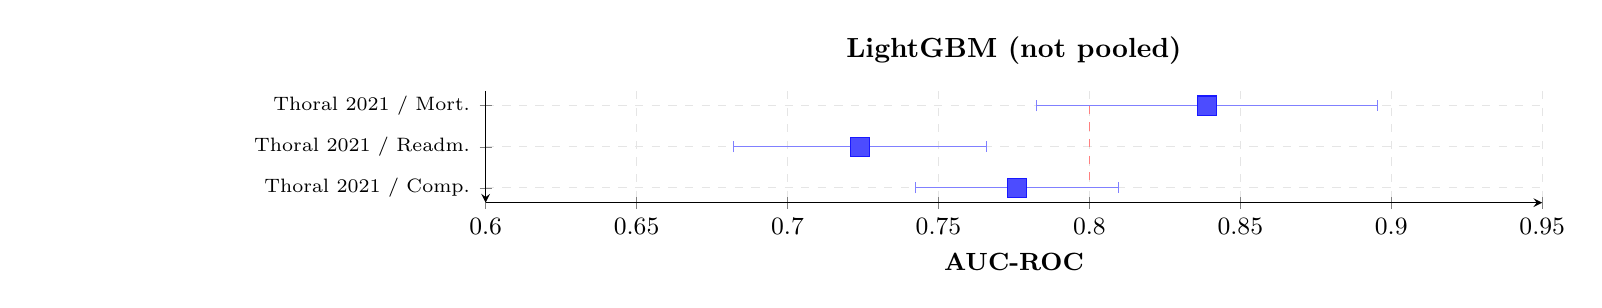
\begin{tikzpicture}[scale=1.0, every node/.style={scale=1.0}]
\begin{axis}[
    width=15cm, height=3.0cm,
    symbolic y coords={
        {Thoral 2021 / Mort.},
        {Thoral 2021 / Readm.},
        {Thoral 2021 / Comp.}
    },
    ytick=data,
    y dir=reverse,
    xmin=0.60, xmax=0.95,
    xlabel={AUC-ROC},
    xlabel style={font=\small\bfseries},
    yticklabel style={font=\scriptsize, text width=5.5cm, align=right},
    xticklabel style={font=\small},
    grid=major,
    grid style={dashed, gray!20},
    axis lines=left,
    clip=false,
    enlarge y limits=0.18,
    title={\textbf{LightGBM (not pooled)}},
    title style={font=\normalsize},
]

\draw[red!50, dashed, thin] (axis cs:0.80,{Thoral 2021 / Mort.}) -- (axis cs:0.80,{Thoral 2021 / Comp.});

\addplot[only marks, mark=none,
    error bars/.cd, x dir=both, x explicit, error bar style={thin, blue!50}]
    coordinates {
(0.839,{Thoral 2021 / Mort.}) +- (0.0565,0)
(0.724,{Thoral 2021 / Readm.}) +- (0.0420,0)
(0.776,{Thoral 2021 / Comp.}) +- (0.0335,0)
    };
\addplot[only marks, mark=square*, fill=blue!70, mark size=3.5pt, draw=blue!90] coordinates {(0.839,{Thoral 2021 / Mort.}) (0.724,{Thoral 2021 / Readm.}) (0.776,{Thoral 2021 / Comp.})};

\end{axis}
\end{tikzpicture}
\caption{Forest plot --- LightGBM: a single study (Thoral et al.~\cite{Thoral2021})
contributes all three outcomes, so none is pooled ($k=1$ each); previously reported as a
single pooled value (0.777) that mixed all three outcomes.}
\label{fig:fp_lightgbm}
\end{figure}
\end{landscape}

\newpage

\begin{landscape}
\subsection{CTCL (2 entries, 1 study): excluded from pooling}

\begin{figure}[H]
\centering
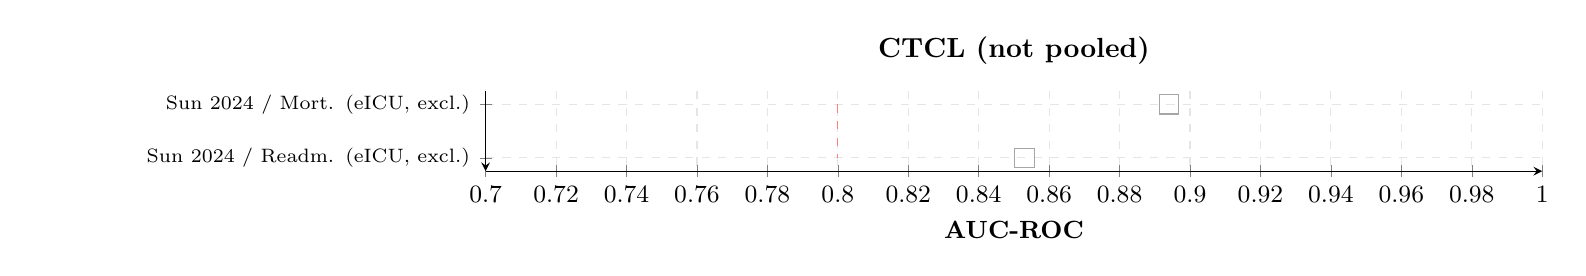
\begin{tikzpicture}[scale=1.0, every node/.style={scale=1.0}]
\begin{axis}[
    width=15cm, height=2.6cm,
    symbolic y coords={
        {Sun 2024 / Mort. (eICU, excl.)},
        {Sun 2024 / Readm. (eICU, excl.)}
    },
    ytick=data,
    y dir=reverse,
    xmin=0.70, xmax=1.00,
    xlabel={AUC-ROC},
    xlabel style={font=\small\bfseries},
    yticklabel style={font=\scriptsize, text width=5.5cm, align=right},
    xticklabel style={font=\small},
    grid=major,
    grid style={dashed, gray!20},
    axis lines=left,
    clip=false,
    enlarge y limits=0.25,
    title={\textbf{CTCL (not pooled)}},
    title style={font=\normalsize},
]

\draw[red!50, dashed, thin] (axis cs:0.80,{Sun 2024 / Mort. (eICU, excl.)}) -- (axis cs:0.80,{Sun 2024 / Readm. (eICU, excl.)});

\addplot[only marks, mark=square, draw=gray!70, mark size=3.5pt] coordinates {
(0.894,{Sun 2024 / Mort. (eICU, excl.)}) (0.853,{Sun 2024 / Readm. (eICU, excl.)})
};

\end{axis}
\end{tikzpicture}
\caption{Forest plot --- CTCL: both estimates are from Sun M. et al.~\cite{Sun2024}, excluded
from AUC-ROC pooling (main text, Section~2.10.4: no event count reported, and independent
evidence from the study's own AUC-PRC values indicates an atypically high evaluation-cohort
prevalence). Previously reported as a pooled value (0.874) mixing mortality and readmission
from a study now excluded entirely.}
\label{fig:fp_ctcl}
\end{figure}
\end{landscape}

\begin{landscape}
\subsection{GRU + Attention (2 entries, 1 study)}

\begin{figure}[H]
\centering
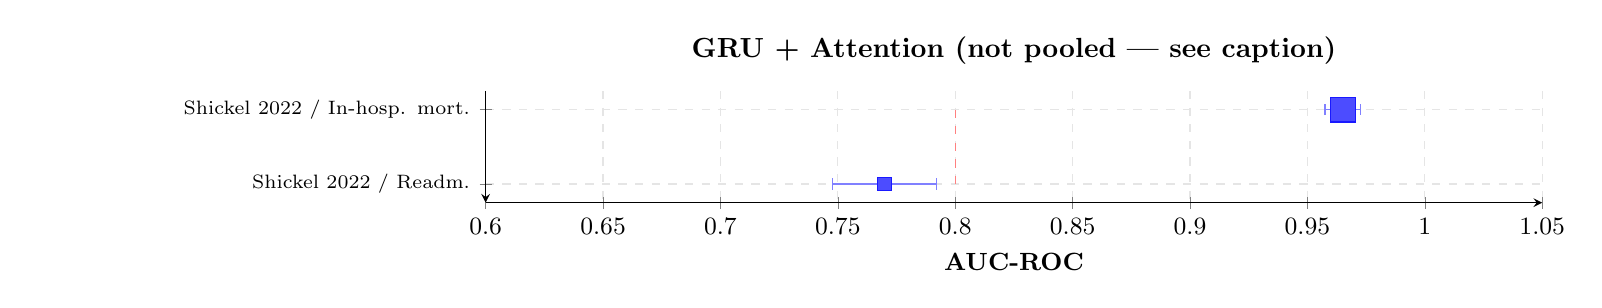
\begin{tikzpicture}[scale=1.0, every node/.style={scale=1.0}]
\begin{axis}[
    width=15cm, height=3.0cm,
    symbolic y coords={
        {Shickel 2022 / In-hosp. mort.},
        {Shickel 2022 / Readm.}
    },
    ytick=data,
    y dir=reverse,
    xmin=0.60, xmax=1.05,
    xlabel={AUC-ROC},
    xlabel style={font=\small\bfseries},
    yticklabel style={font=\scriptsize, text width=5.5cm, align=right},
    xticklabel style={font=\small},
    grid=major,
    grid style={dashed, gray!20},
    axis lines=left,
    clip=false,
    enlarge y limits=0.25,
    title={\textbf{GRU + Attention (not pooled --- see caption)}},
    title style={font=\normalsize},
]

\draw[red!50, dashed, thin] (axis cs:0.80,{Shickel 2022 / In-hosp. mort.}) -- (axis cs:0.80,{Shickel 2022 / Readm.});

\addplot[only marks, mark=none,
    error bars/.cd, x dir=both, x explicit, error bar style={thin, blue!50}]
    coordinates {
(0.965,{Shickel 2022 / In-hosp. mort.}) +- (0.0075,0)
(0.770,{Shickel 2022 / Readm.}) +- (0.0222,0)
    };
% Markers with size proportional to each estimate's inverse-variance weight
% (weight ~ 1/SE^2); despite k=2, the SEs differ substantially (0.0075 vs.
% 0.0222), so the sizes are not equal
\addplot[only marks, mark=square*, fill=blue!70, mark size=4.50pt, draw=blue!90] coordinates {(0.965,{Shickel 2022 / In-hosp. mort.})};
\addplot[only marks, mark=square*, fill=blue!70, mark size=2.50pt, draw=blue!90] coordinates {(0.770,{Shickel 2022 / Readm.})};

\end{axis}
\end{tikzpicture}
\caption{Forest plot --- GRU + Attention. This model-family/outcome pair is no longer
pooled (main text, Section~2.10.4): both entries come from a single study
(Shickel et al.~\cite{Shickel2022}) and represent two distinct outcomes (in-hospital
mortality and readmission), so stratifying by outcome (Table~\ref{tab:sscale}
methodology) leaves only $k=1$ estimate per outcome. The two individual estimates are
shown above without a pooled diamond; the previously reported pooled value (0.868, 95\%
CI 0.677--1.000) mixed these two outcomes and produced a confidence interval exceeding
the mathematically admissible upper bound of 1.000, both of which are resolved by this
correction.}
\label{fig:fp_gruatt}
\end{figure}
\end{landscape}

\begin{landscape}
\subsection{GRU (2 entries, 1 study)}

\begin{figure}[H]
\centering
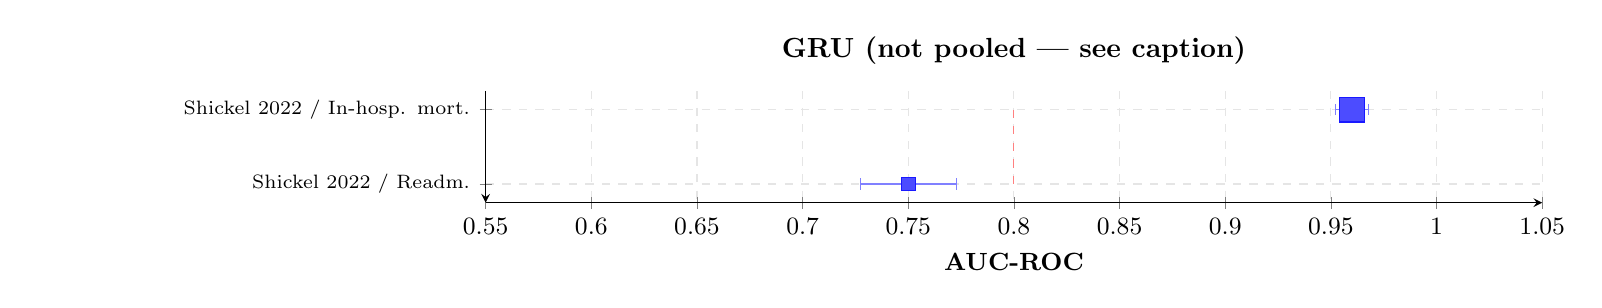
\begin{tikzpicture}[scale=1.0, every node/.style={scale=1.0}]
\begin{axis}[
    width=15cm, height=3.0cm,
    symbolic y coords={
        {Shickel 2022 / In-hosp. mort.},
        {Shickel 2022 / Readm.}
    },
    ytick=data,
    y dir=reverse,
    xmin=0.55, xmax=1.05,
    xlabel={AUC-ROC},
    xlabel style={font=\small\bfseries},
    yticklabel style={font=\scriptsize, text width=5.5cm, align=right},
    xticklabel style={font=\small},
    grid=major,
    grid style={dashed, gray!20},
    axis lines=left,
    clip=false,
    enlarge y limits=0.25,
    title={\textbf{GRU (not pooled --- see caption)}},
    title style={font=\normalsize},
]

\draw[red!50, dashed, thin] (axis cs:0.80,{Shickel 2022 / In-hosp. mort.}) -- (axis cs:0.80,{Shickel 2022 / Readm.});

\addplot[only marks, mark=none,
    error bars/.cd, x dir=both, x explicit, error bar style={thin, blue!50}]
    coordinates {
(0.960,{Shickel 2022 / In-hosp. mort.}) +- (0.0080,0)
(0.750,{Shickel 2022 / Readm.}) +- (0.0227,0)
    };
% Markers with size proportional to each estimate's inverse-variance weight
% (weight ~ 1/SE^2); despite k=2, the SEs differ substantially (0.0080 vs.
% 0.0227), so the sizes are not equal
\addplot[only marks, mark=square*, fill=blue!70, mark size=4.50pt, draw=blue!90] coordinates {(0.960,{Shickel 2022 / In-hosp. mort.})};
\addplot[only marks, mark=square*, fill=blue!70, mark size=2.50pt, draw=blue!90] coordinates {(0.750,{Shickel 2022 / Readm.})};

\end{axis}
\end{tikzpicture}
\caption{Forest plot --- GRU. This model-family/outcome pair is no longer pooled (main
text, Section~2.10.4): both entries come from a single study
(Shickel et al.~\cite{Shickel2022}) and represent two distinct outcomes (in-hospital
mortality and readmission), so stratifying by outcome leaves only $k=1$ estimate per
outcome. The two individual estimates are shown above without a pooled diamond; the
previously reported pooled value (0.855, 95\% CI 0.649--1.000) mixed these two outcomes
and produced a confidence interval exceeding the mathematically admissible upper bound of
1.000, both of which are resolved by this correction.}
\label{fig:fp_gru}
\end{figure}
\end{landscape}

\newpage

\begin{landscape}
\subsection{CatBoost (2 entries, 1 study): not pooled}

\begin{figure}[H]
\centering
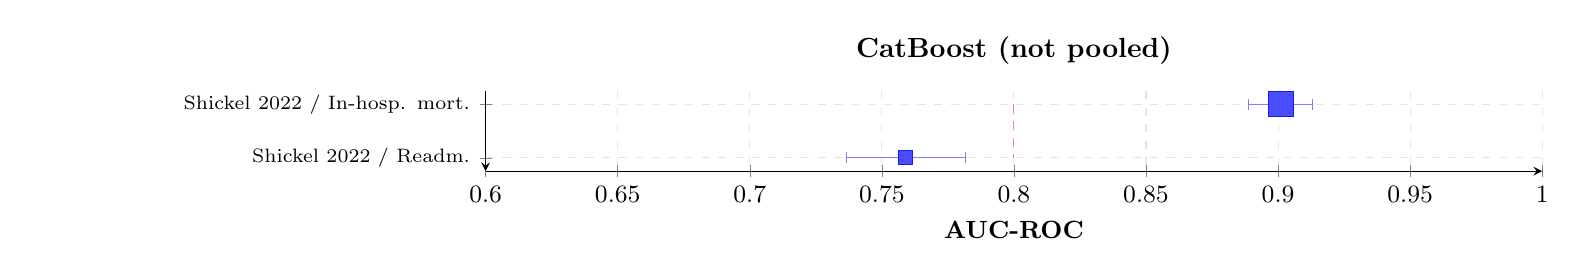
\begin{tikzpicture}[scale=1.0, every node/.style={scale=1.0}]
\begin{axis}[
    width=15cm, height=2.6cm,
    symbolic y coords={
        {Shickel 2022 / In-hosp. mort.},
        {Shickel 2022 / Readm.}
    },
    ytick=data,
    y dir=reverse,
    xmin=0.60, xmax=1.00,
    xlabel={AUC-ROC},
    xlabel style={font=\small\bfseries},
    yticklabel style={font=\scriptsize, text width=5.5cm, align=right},
    xticklabel style={font=\small},
    grid=major,
    grid style={dashed, gray!20},
    axis lines=left,
    clip=false,
    enlarge y limits=0.25,
    title={\textbf{CatBoost (not pooled)}},
    title style={font=\normalsize},
]

\draw[red!50, dashed, thin] (axis cs:0.80,{Shickel 2022 / In-hosp. mort.}) -- (axis cs:0.80,{Shickel 2022 / Readm.});

\addplot[only marks, mark=none,
    error bars/.cd, x dir=both, x explicit, error bar style={thin, blue!50}]
    coordinates {
(0.901,{Shickel 2022 / In-hosp. mort.}) +- (0.0121,0)
(0.759,{Shickel 2022 / Readm.}) +- (0.0225,0)
    };
% Markers with size proportional to each estimate's inverse-variance weight
% (weight ~ 1/SE^2); despite k=2, the SEs differ substantially (0.0121 vs.
% 0.0225), so the sizes are not equal
\addplot[only marks, mark=square*, fill=blue!70, mark size=4.50pt, draw=blue!90] coordinates {(0.901,{Shickel 2022 / In-hosp. mort.})};
\addplot[only marks, mark=square*, fill=blue!70, mark size=2.50pt, draw=blue!90] coordinates {(0.759,{Shickel 2022 / Readm.})};

\end{axis}
\end{tikzpicture}
\caption{Forest plot --- CatBoost: both entries come from a single study
(Shickel et al.~\cite{Shickel2022}) and represent two distinct outcomes (in-hospital
mortality and readmission), so stratifying by outcome leaves only $k=1$ estimate per
outcome. Previously reported as a pooled value (0.830, 95\% CI 0.691--0.969) mixing
these two outcomes.}
\label{fig:fp_catboost}
\end{figure}
\end{landscape}

\newpage

\begin{landscape}
\subsection{Ensemble (1 entry, 1 study)}

\begin{figure}[H]
\centering
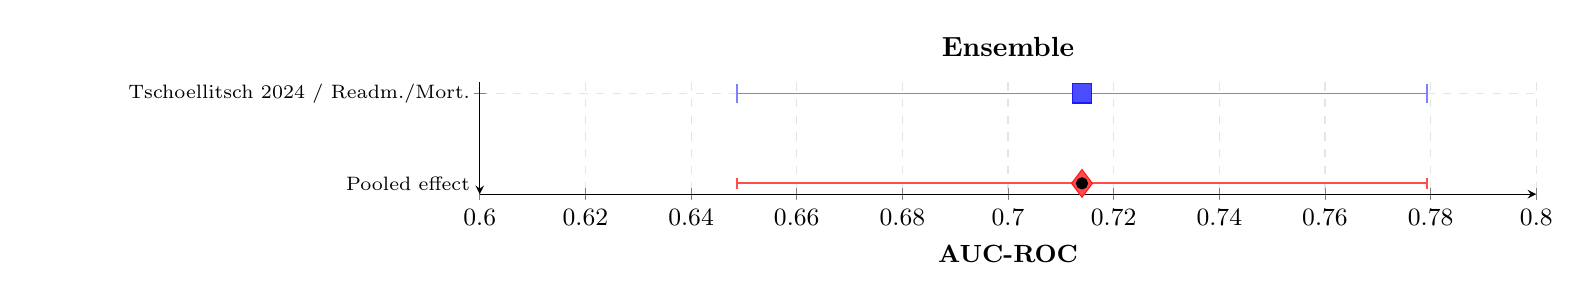
\begin{tikzpicture}[scale=1.0, every node/.style={scale=1.0}]
\begin{axis}[
    width=15cm, height=3.0cm,
    symbolic y coords={
        {Tschoellitsch 2024 / Readm./Mort.},
        Pooled effect
    },
    ytick=data,
    y dir=reverse,
    yticklabel=\empty,
    xmin=0.60, xmax=0.80,
    xlabel={AUC-ROC},
    xlabel style={font=\small\bfseries},
    xticklabel style={font=\small},
    grid=major,
    grid style={dashed, gray!20},
    axis lines=left,
    clip=false,
    enlarge y limits=0.12,
    title={\textbf{Ensemble}},
    title style={font=\normalsize},
]
\node[anchor=east, font=\scriptsize, text width=5.5cm, align=right] at (axis cs:0.60,{Tschoellitsch 2024 / Readm./Mort.}) {Tschoellitsch 2024 / Readm./Mort.};
\node[anchor=east, font=\scriptsize, text width=5.5cm, align=right] at (axis cs:0.60,Pooled effect) {Pooled effect};

\addplot[only marks, mark=square*, fill=blue!70, mark size=3.5pt, draw=blue!90,
    error bars/.cd, x dir=both, x explicit, error bar style={thin, blue!50}]
    coordinates {
(0.714,{Tschoellitsch 2024 / Readm./Mort.}) +- (0.0653,0)
    };

\addplot[only marks, mark=diamond*, fill=red!70, mark size=5pt, draw=red!90]
    coordinates {(0.714,{Pooled effect})};
\addplot[only marks, mark=none, forget plot,
    error bars/.cd, x dir=both, x explicit, error bar style={thick, red!70}]
    coordinates {(0.714,{Pooled effect}) +- (0.0653,0)};

\end{axis}
\end{tikzpicture}
\caption{Forest plot --- Ensemble (single estimate, $k=1$; not a meta-analytic pool).
0.714 (95\% CI: 0.649--0.779), standard error corrected for Tschoellitsch et
al.~\cite{Tschoellitsch2024}'s actual evaluation-set size (25\% of the internal cohort;
main text, Section~2.10.4).}
\label{fig:fp_ensemble}
\end{figure}
\end{landscape}

\newpage

\begin{landscape}
\subsection{AdaBoost (1 entry, 1 study)}

\begin{figure}[H]
\centering
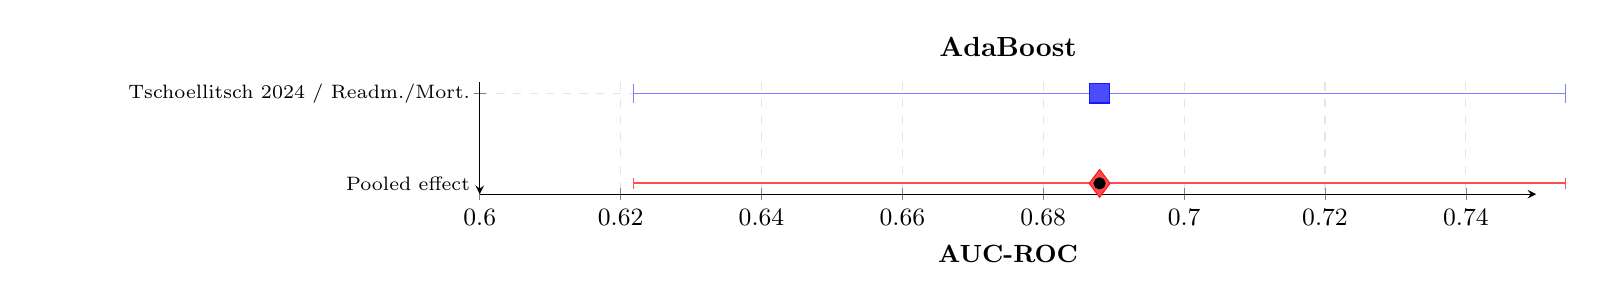
\begin{tikzpicture}[scale=1.0, every node/.style={scale=1.0}]
\begin{axis}[
    width=15cm, height=3.0cm,
    symbolic y coords={
        {Tschoellitsch 2024 / Readm./Mort.},
        Pooled effect
    },
    ytick=data,
    y dir=reverse,
    yticklabel=\empty,
    xmin=0.60, xmax=0.75,
    xlabel={AUC-ROC},
    xlabel style={font=\small\bfseries},
    xticklabel style={font=\small},
    grid=major,
    grid style={dashed, gray!20},
    axis lines=left,
    clip=false,
    enlarge y limits=0.12,
    title={\textbf{AdaBoost}},
    title style={font=\normalsize},
]
\node[anchor=east, font=\scriptsize, text width=5.5cm, align=right] at (axis cs:0.60,{Tschoellitsch 2024 / Readm./Mort.}) {Tschoellitsch 2024 / Readm./Mort.};
\node[anchor=east, font=\scriptsize, text width=5.5cm, align=right] at (axis cs:0.60,Pooled effect) {Pooled effect};

\addplot[only marks, mark=square*, fill=blue!70, mark size=3.5pt, draw=blue!90,
    error bars/.cd, x dir=both, x explicit, error bar style={thin, blue!50}]
    coordinates {
(0.688,{Tschoellitsch 2024 / Readm./Mort.}) +- (0.0662,0)
    };

\addplot[only marks, mark=diamond*, fill=red!70, mark size=5pt, draw=red!90]
    coordinates {(0.688,{Pooled effect})};
\addplot[only marks, mark=none, forget plot,
    error bars/.cd, x dir=both, x explicit, error bar style={thick, red!70}]
    coordinates {(0.688,{Pooled effect}) +- (0.0662,0)};

\end{axis}
\end{tikzpicture}
\caption{Forest plot --- AdaBoost (single estimate, $k=1$; not a meta-analytic pool).
0.688 (95\% CI: 0.622--0.754), standard error corrected for Tschoellitsch et
al.~\cite{Tschoellitsch2024}'s actual evaluation-set size (main text, Section~2.10.4).}
\label{fig:fp_adaboost}
\end{figure}
\end{landscape}

\newpage

\begin{landscape}
\subsection{Naive Bayes (1 entry, 1 study)}

\begin{figure}[H]
\centering
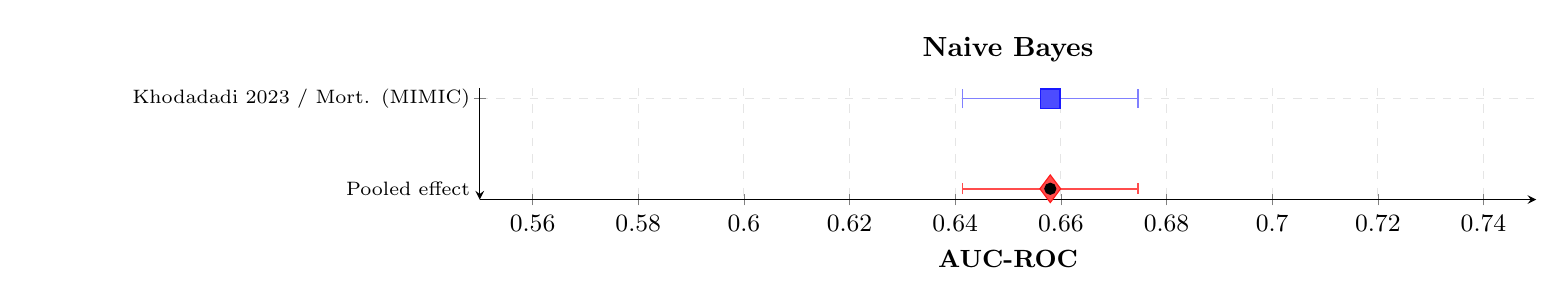
\begin{tikzpicture}[scale=1.0, every node/.style={scale=1.0}]
\begin{axis}[
    width=15cm, height=3.0cm,
    symbolic y coords={
        {Khodadadi 2023 / Mort. (MIMIC)},
        Pooled effect
    },
    ytick=data,
    y dir=reverse,
    yticklabel=\empty,
    xmin=0.55, xmax=0.75,
    xlabel={AUC-ROC},
    xlabel style={font=\small\bfseries},
    xticklabel style={font=\small},
    grid=major,
    grid style={dashed, gray!20},
    axis lines=left,
    clip=false,
    enlarge y limits=0.12,
    title={\textbf{Naive Bayes}},
    title style={font=\normalsize},
]
\node[anchor=east, font=\scriptsize, text width=5.5cm, align=right] at (axis cs:0.55,{Khodadadi 2023 / Mort. (MIMIC)}) {Khodadadi 2023 / Mort. (MIMIC)};
\node[anchor=east, font=\scriptsize, text width=5.5cm, align=right] at (axis cs:0.55,Pooled effect) {Pooled effect};

\addplot[only marks, mark=square*, fill=blue!70, mark size=3.5pt, draw=blue!90,
    error bars/.cd, x dir=both, x explicit, error bar style={thin, blue!50}]
    coordinates {
(0.658,{Khodadadi 2023 / Mort. (MIMIC)}) +- (0.0166,0)
    };

\addplot[only marks, mark=diamond*, fill=red!70, mark size=5pt, draw=red!90]
    coordinates {(0.658,{Pooled effect})};
\addplot[only marks, mark=none, forget plot,
    error bars/.cd, x dir=both, x explicit, error bar style={thick, red!70}]
    coordinates {(0.658,{Pooled effect}) +- (0.0166,0)};

\end{axis}
\end{tikzpicture}
\caption{Forest plot --- Naive Bayes (single estimate, $k=1$; not a meta-analytic pool).
0.658 (95\% CI: 0.641--0.675), standard error corrected for Khodadadi et
al.~\cite{Khodadadi2023}'s actual evaluation-set size (25\% split; main text,
Section~2.10.4).}
\label{fig:fp_nb}
\end{figure}
\end{landscape}

\newpage

\begin{landscape}
\subsection{K-Nearest Neighbors (1 entry, 1 study)}

\begin{figure}[H]
\centering
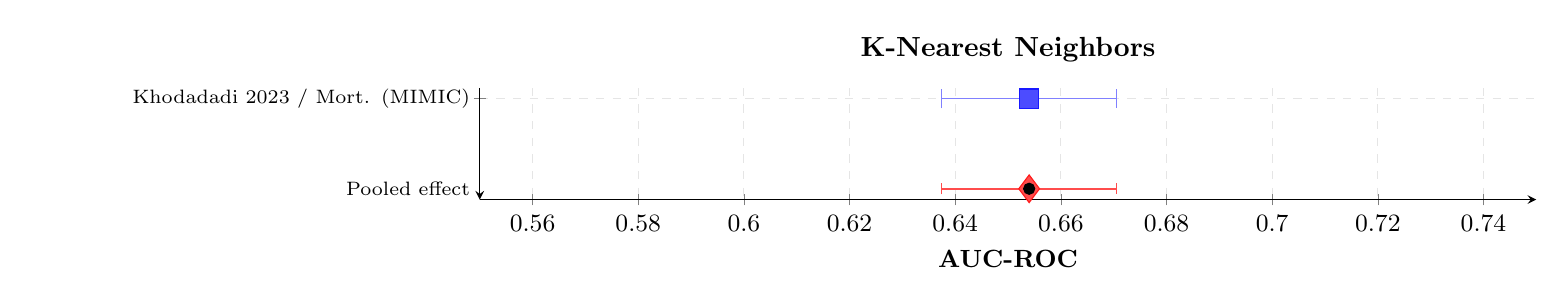
\begin{tikzpicture}[scale=1.0, every node/.style={scale=1.0}]
\begin{axis}[
    width=15cm, height=3.0cm,
    symbolic y coords={
        {Khodadadi 2023 / Mort. (MIMIC)},
        Pooled effect
    },
    ytick=data,
    y dir=reverse,
    yticklabel=\empty,
    xmin=0.55, xmax=0.75,
    xlabel={AUC-ROC},
    xlabel style={font=\small\bfseries},
    xticklabel style={font=\small},
    grid=major,
    grid style={dashed, gray!20},
    axis lines=left,
    clip=false,
    enlarge y limits=0.12,
    title={\textbf{K-Nearest Neighbors}},
    title style={font=\normalsize},
]
\node[anchor=east, font=\scriptsize, text width=5.5cm, align=right] at (axis cs:0.55,{Khodadadi 2023 / Mort. (MIMIC)}) {Khodadadi 2023 / Mort. (MIMIC)};
\node[anchor=east, font=\scriptsize, text width=5.5cm, align=right] at (axis cs:0.55,Pooled effect) {Pooled effect};

\addplot[only marks, mark=square*, fill=blue!70, mark size=3.5pt, draw=blue!90,
    error bars/.cd, x dir=both, x explicit, error bar style={thin, blue!50}]
    coordinates {
(0.654,{Khodadadi 2023 / Mort. (MIMIC)}) +- (0.0166,0)
    };

\addplot[only marks, mark=diamond*, fill=red!70, mark size=5pt, draw=red!90]
    coordinates {(0.654,{Pooled effect})};
\addplot[only marks, mark=none, forget plot,
    error bars/.cd, x dir=both, x explicit, error bar style={thick, red!70}]
    coordinates {(0.654,{Pooled effect}) +- (0.0166,0)};

\end{axis}
\end{tikzpicture}
\caption{Forest plot --- K-Nearest Neighbors (single estimate, $k=1$; not a
meta-analytic pool). 0.654 (95\% CI: 0.637--0.671), standard error corrected for
Khodadadi et al.~\cite{Khodadadi2023}'s actual evaluation-set size (main text,
Section~2.10.4).}
\label{fig:fp_knn}
\end{figure}
\end{landscape}

% ==================================================================
\newpage
\section{Precision--Recall Metrics}

\subsection{Global Forest Plots}

\begin{figure}[H]
\centering
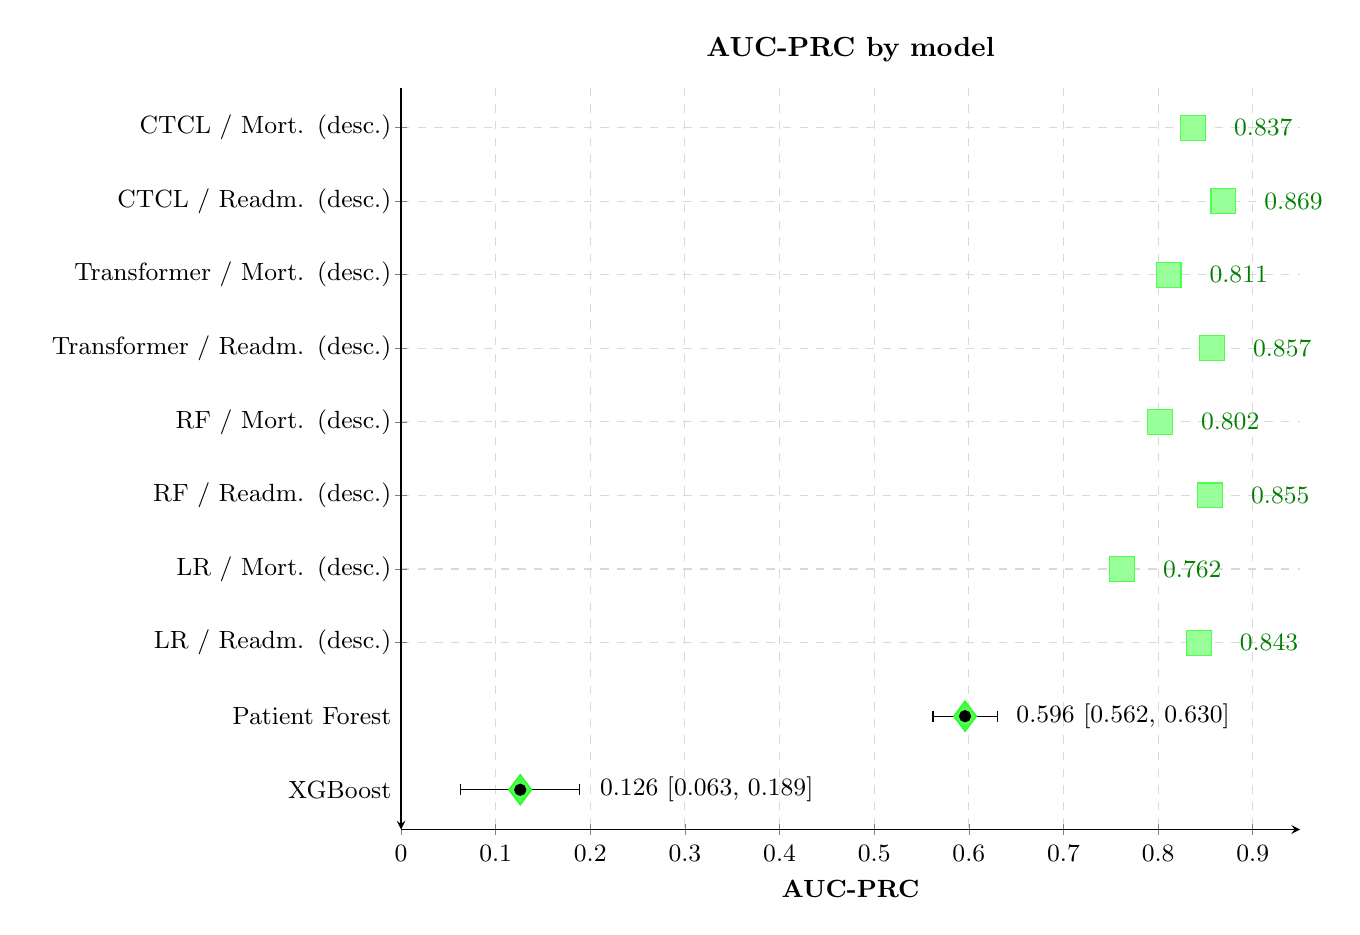
\begin{tikzpicture}
\begin{axis}[
    width=13cm, height=11cm,
    symbolic y coords={
        {CTCL / Mort. (desc.)},
        {CTCL / Readm. (desc.)},
        {Transformer / Mort. (desc.)},
        {Transformer / Readm. (desc.)},
        {RF / Mort. (desc.)},
        {RF / Readm. (desc.)},
        {LR / Mort. (desc.)},
        {LR / Readm. (desc.)},
        {Patient Forest},
        {XGBoost}
    },
    ytick=data,
    y dir=reverse,
    yticklabel=\empty,
    xmin=0.00, xmax=0.95,
    xlabel={AUC-PRC}, xlabel style={font=\small\bfseries},
    xticklabel style={font=\small},
    grid=major, grid style={dashed, gray!30},
    axis lines=left, clip=false, enlarge y limits=0.06,
    title={\textbf{AUC-PRC by model}}, title style={font=\normalsize},
]
\node[anchor=east, font=\small, text width=4.5cm, align=right] at (axis cs:0.00,{CTCL / Mort. (desc.)}) {CTCL / Mort. (desc.)};
\node[anchor=east, font=\small, text width=4.5cm, align=right] at (axis cs:0.00,{CTCL / Readm. (desc.)}) {CTCL / Readm. (desc.)};
\node[anchor=east, font=\small, text width=4.5cm, align=right] at (axis cs:0.00,{Transformer / Mort. (desc.)}) {Transformer / Mort. (desc.)};
\node[anchor=east, font=\small, text width=4.5cm, align=right] at (axis cs:0.00,{Transformer / Readm. (desc.)}) {Transformer / Readm. (desc.)};
\node[anchor=east, font=\small, text width=4.5cm, align=right] at (axis cs:0.00,{RF / Mort. (desc.)}) {RF / Mort. (desc.)};
\node[anchor=east, font=\small, text width=4.5cm, align=right] at (axis cs:0.00,{RF / Readm. (desc.)}) {RF / Readm. (desc.)};
\node[anchor=east, font=\small, text width=4.5cm, align=right] at (axis cs:0.00,{LR / Mort. (desc.)}) {LR / Mort. (desc.)};
\node[anchor=east, font=\small, text width=4.5cm, align=right] at (axis cs:0.00,{LR / Readm. (desc.)}) {LR / Readm. (desc.)};
\node[anchor=east, font=\small, text width=4.5cm, align=right] at (axis cs:0.00,{Patient Forest}) {Patient Forest};
\node[anchor=east, font=\small, text width=4.5cm, align=right] at (axis cs:0.00,{XGBoost}) {XGBoost};
% CTCL/Transformer/RF/LR (desc.): Sun M. et al. is the sole source, shown
% per-outcome descriptively (k=1, no diamond) -- see Table S-subgroup-pr note
\addplot[only marks, mark=square*, mark size=4.5pt, fill=green!40, draw=green!70]
    coordinates {
(0.837,{CTCL / Mort. (desc.)})
(0.869,{CTCL / Readm. (desc.)})
(0.811,{Transformer / Mort. (desc.)})
(0.857,{Transformer / Readm. (desc.)})
(0.802,{RF / Mort. (desc.)})
(0.855,{RF / Readm. (desc.)})
(0.762,{LR / Mort. (desc.)})
(0.843,{LR / Readm. (desc.)})
    };
% Patient Forest and XGBoost: genuine pooled diamonds (unaffected by this revision)
\addplot[only marks, mark=diamond*, mark size=5.5pt, fill=green!70, draw=green!90]
    coordinates {
(0.596,{Patient Forest})
(0.126,{XGBoost})
    };
\addplot[only marks, mark=none, forget plot,
    error bars/.cd, x dir=both, x explicit, error bar style={thin, black}]
    coordinates {
(0.596,{Patient Forest}) +- (0.0339,0)
(0.126,{XGBoost}) +- (0.0627,0)
    };
\node[anchor=west, font=\small, text=green!50!black] at (axis cs:0.870,{CTCL / Mort. (desc.)}) {0.837};
\node[anchor=west, font=\small, text=green!50!black] at (axis cs:0.902,{CTCL / Readm. (desc.)}) {0.869};
\node[anchor=west, font=\small, text=green!50!black] at (axis cs:0.844,{Transformer / Mort. (desc.)}) {0.811};
\node[anchor=west, font=\small, text=green!50!black] at (axis cs:0.890,{Transformer / Readm. (desc.)}) {0.857};
\node[anchor=west, font=\small, text=green!50!black] at (axis cs:0.835,{RF / Mort. (desc.)}) {0.802};
\node[anchor=west, font=\small, text=green!50!black] at (axis cs:0.888,{RF / Readm. (desc.)}) {0.855};
\node[anchor=west, font=\small, text=green!50!black] at (axis cs:0.795,{LR / Mort. (desc.)}) {0.762};
\node[anchor=west, font=\small, text=green!50!black] at (axis cs:0.876,{LR / Readm. (desc.)}) {0.843};
\node[anchor=west, font=\small] at (axis cs:0.640,{Patient Forest}) {0.596 [0.562, 0.630]};
\node[anchor=west, font=\small] at (axis cs:0.200,{XGBoost}) {0.126 [0.063, 0.189]};
\end{axis}
\end{tikzpicture}
\caption{Global AUC-PRC forest plot by model. Patient Forest and XGBoost show genuine
pooled effects (random-effects, inverse-variance weighting). CTCL, Transformer, RF, and
LR are Sun M. et al. (2024)'s sole-source estimates, shown per outcome descriptively
(square markers, no diamond) rather than pooled across mortality and readmission --
this replaces an earlier version of this figure that pooled each of these four models
into one number mixing both outcomes (e.g., CTCL was previously reported as 0.874).}
\label{fig:fp_global_auprc}
\end{figure}

\begin{figure}[H]
\centering
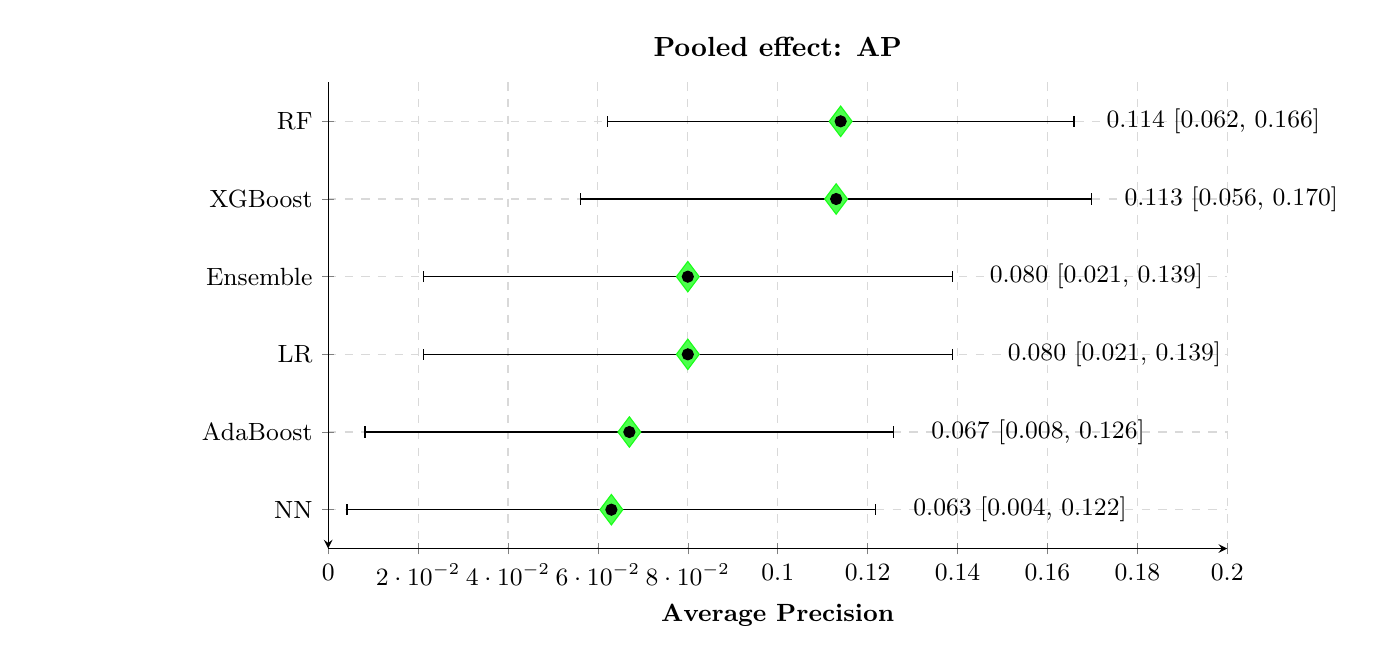
\begin{tikzpicture}
\begin{axis}[
    width=13cm, height=7.5cm,
    symbolic y coords={
        {RF},
        {XGBoost},
        {Ensemble},
        {LR},
        {AdaBoost},
        {NN}
    },
    ytick=data,
    y dir=reverse,
    xmin=0.00, xmax=0.20,
    xlabel={Average Precision}, xlabel style={font=\small\bfseries},
    yticklabel style={font=\small, text width=3.5cm, align=right},
    xticklabel style={font=\small},
    grid=major, grid style={dashed, gray!30},
    axis lines=left, clip=false, enlarge y limits=0.10,
    title={\textbf{Pooled effect: AP}}, title style={font=\normalsize},
]
\addplot[only marks, mark=diamond*, mark size=5.5pt, fill=green!70, draw=green!90]
    coordinates {
(0.114,{RF})
(0.113,{XGBoost})
(0.080,{Ensemble})
(0.080,{LR})
(0.067,{AdaBoost})
(0.063,{NN})
    };
\addplot[only marks, mark=none, forget plot,
    error bars/.cd, x dir=both, x explicit, error bar style={thin, black}]
    coordinates {
(0.114,{RF}) +- (0.0519,0)
(0.113,{XGBoost}) +- (0.0568,0)
(0.080,{Ensemble}) +- (0.0588,0)
(0.080,{LR}) +- (0.0588,0)
(0.067,{AdaBoost}) +- (0.0588,0)
(0.063,{NN}) +- (0.0588,0)
    };
\node[anchor=west, font=\small] at (axis cs:0.171,{RF}) {0.114 [0.062, 0.166]};
\node[anchor=west, font=\small] at (axis cs:0.175,{XGBoost}) {0.113 [0.056, 0.170]};
\node[anchor=west, font=\small] at (axis cs:0.145,{Ensemble}) {0.080 [0.021, 0.139]};
\node[anchor=west, font=\small] at (axis cs:0.149,{LR}) {0.080 [0.021, 0.139]};
\node[anchor=west, font=\small] at (axis cs:0.132,{AdaBoost}) {0.067 [0.008, 0.126]};
\node[anchor=west, font=\small] at (axis cs:0.128,{NN}) {0.063 [0.004, 0.122]};
\end{axis}
\end{tikzpicture}
\caption{Global AP forest plot by model (random-effects, inverse-variance weighting).}
\label{fig:fp_global_ap}
\end{figure}

\begin{landscape}
\section{Individual Precision--Recall Forest Plots by Model}

\subsection{Patient Forest --- AUPR/AUPRC (3 entries, 1 study)}

\begin{figure}[H]
\centering
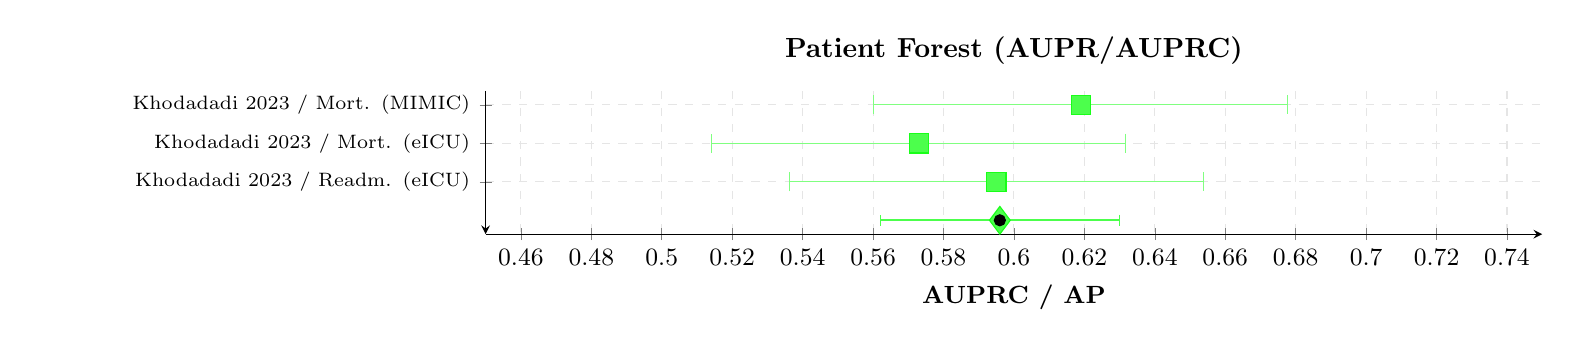
\begin{tikzpicture}[scale=1.0, every node/.style={scale=1.0}]
\begin{axis}[
    width=15cm, height=3.4cm,
    symbolic y coords={
        {Khodadadi 2023 / Mort. (MIMIC)},
        {Khodadadi 2023 / Mort. (eICU)},
        {Khodadadi 2023 / Readm. (eICU)},
        Pooled effect
    },
    ytick=data,
    y dir=reverse,
    xmin=0.45, xmax=0.75,
    xlabel={AUPRC / AP},
    xlabel style={font=\small\bfseries},
    yticklabel style={font=\scriptsize, text width=5.5cm, align=right},
    xticklabel style={font=\small},
    grid=major,
    grid style={dashed, gray!20},
    axis lines=left,
    clip=false,
    enlarge y limits=0.12,
    title={\textbf{Patient Forest (AUPR/AUPRC)}},
    title style={font=\normalsize},
]

\addplot[only marks, mark=square*, fill=green!70, mark size=3.5pt, draw=green!90,
    error bars/.cd, x dir=both, x explicit, error bar style={thin, green!50}]
    coordinates {
(0.619,{Khodadadi 2023 / Mort. (MIMIC)}) +- (0.0588,0)
(0.573,{Khodadadi 2023 / Mort. (eICU)}) +- (0.0588,0)
(0.595,{Khodadadi 2023 / Readm. (eICU)}) +- (0.0588,0)
    };

\addplot[only marks, mark=diamond*, fill=green!70, mark size=5pt, draw=green!90]
    coordinates {(0.596,{Pooled effect})};
\addplot[only marks, mark=none, forget plot,
    error bars/.cd, x dir=both, x explicit, error bar style={thick, green!70}]
    coordinates {(0.596,{Pooled effect}) +- (0.0339,0)};

\end{axis}
\end{tikzpicture}
\caption{PR forest plot --- Patient Forest (AUPR/AUPRC). Pooled effect: 0.596 (95\% CI: 0.562--0.630).}
\label{fig:fp_pr_patientforest}
\end{figure}
\end{landscape}

\begin{landscape}
\subsection{XGBoost --- AUPR/AUPRC (3 entries, 1 study)}

\begin{figure}[H]
\centering
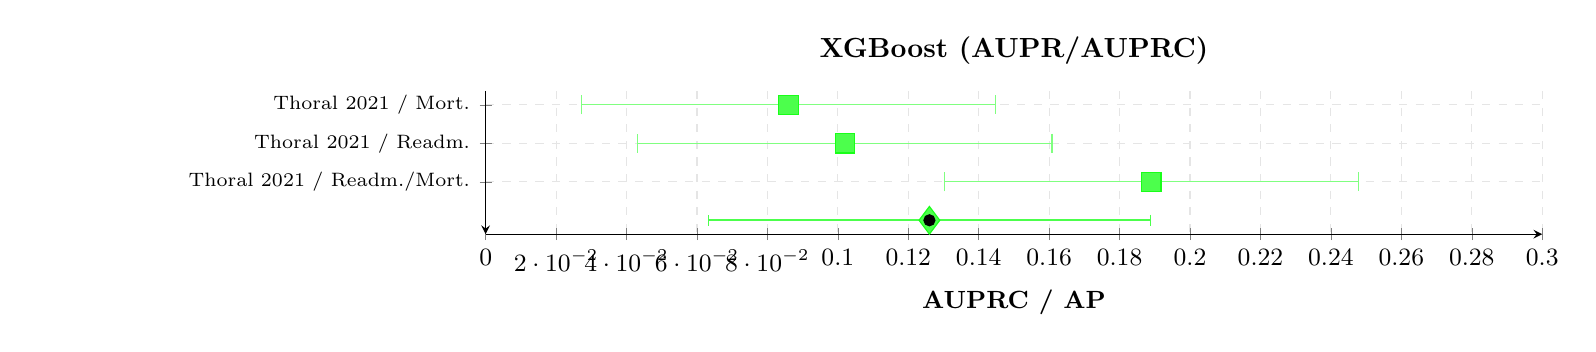
\begin{tikzpicture}[scale=1.0, every node/.style={scale=1.0}]
\begin{axis}[
    width=15cm, height=3.4cm,
    symbolic y coords={
        {Thoral 2021 / Mort.},
        {Thoral 2021 / Readm.},
        {Thoral 2021 / Readm./Mort.},
        Pooled effect
    },
    ytick=data,
    y dir=reverse,
    xmin=0.00, xmax=0.30,
    xlabel={AUPRC / AP},
    xlabel style={font=\small\bfseries},
    yticklabel style={font=\scriptsize, text width=5.5cm, align=right},
    xticklabel style={font=\small},
    grid=major,
    grid style={dashed, gray!20},
    axis lines=left,
    clip=false,
    enlarge y limits=0.12,
    title={\textbf{XGBoost (AUPR/AUPRC)}},
    title style={font=\normalsize},
]

\addplot[only marks, mark=square*, fill=green!70, mark size=3.5pt, draw=green!90,
    error bars/.cd, x dir=both, x explicit, error bar style={thin, green!50}]
    coordinates {
(0.086,{Thoral 2021 / Mort.}) +- (0.0588,0)
(0.102,{Thoral 2021 / Readm.}) +- (0.0588,0)
(0.189,{Thoral 2021 / Readm./Mort.}) +- (0.0588,0)
    };

\addplot[only marks, mark=diamond*, fill=green!70, mark size=5pt, draw=green!90]
    coordinates {(0.126,{Pooled effect})};
\addplot[only marks, mark=none, forget plot,
    error bars/.cd, x dir=both, x explicit, error bar style={thick, green!70}]
    coordinates {(0.126,{Pooled effect}) +- (0.0627,0)};

\end{axis}
\end{tikzpicture}
\caption{PR forest plot --- XGBoost (AUPR/AUPRC). Pooled effect: 0.126 (95\% CI: 0.063--0.188).}
\label{fig:fp_pr_xgboost_auprc}
\end{figure}
\end{landscape}

\newpage

\begin{landscape}
\subsection{CTCL --- AUPR/AUPRC (2 entries, 1 study): not pooled}

\begin{figure}[H]
\centering
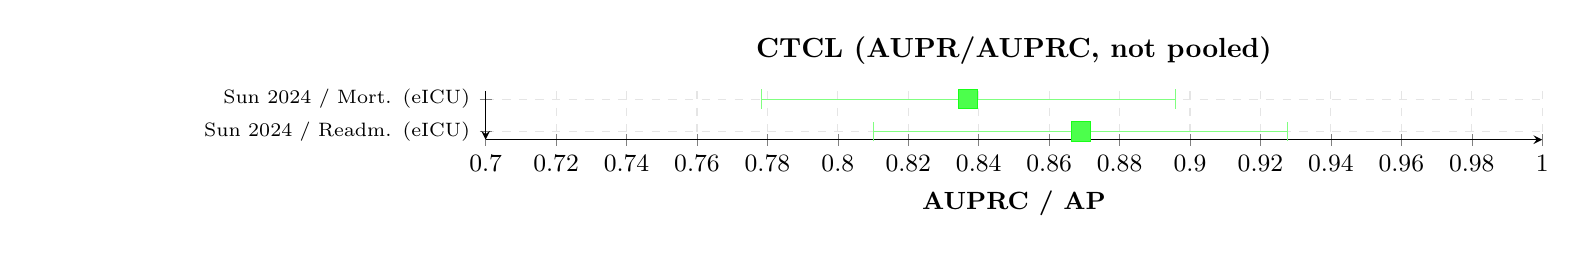
\begin{tikzpicture}[scale=1.0, every node/.style={scale=1.0}]
\begin{axis}[
    width=15cm, height=2.2cm,
    symbolic y coords={
        {Sun 2024 / Mort. (eICU)},
        {Sun 2024 / Readm. (eICU)}
    },
    ytick=data,
    y dir=reverse,
    xmin=0.70, xmax=1.00,
    xlabel={AUPRC / AP},
    xlabel style={font=\small\bfseries},
    yticklabel style={font=\scriptsize, text width=5.5cm, align=right},
    xticklabel style={font=\small},
    grid=major,
    grid style={dashed, gray!20},
    axis lines=left,
    clip=false,
    enlarge y limits=0.25,
    title={\textbf{CTCL (AUPR/AUPRC, not pooled)}},
    title style={font=\normalsize},
]

\addplot[only marks, mark=square*, fill=green!70, mark size=3.5pt, draw=green!90,
    error bars/.cd, x dir=both, x explicit, error bar style={thin, green!50}]
    coordinates {
(0.837,{Sun 2024 / Mort. (eICU)}) +- (0.0588,0)
(0.869,{Sun 2024 / Readm. (eICU)}) +- (0.0588,0)
    };

\end{axis}
\end{tikzpicture}
\caption{PR forest plot --- CTCL (AUPR/AUPRC). Both estimates are from Sun M. et al.~\cite{Sun2024}, the sole source for this model. Unlike this study's AUC-ROC
estimates, these are not excluded for quality reasons (AUC-PRC pooling does not
depend on the missing event counts) but are not pooled because no other study
reports AUC-PRC for CTCL ($k=1$ per outcome); shown per outcome rather than mixed
into one number (main text, Section~2.10.4). See main text Section~4.1 for why
these values should still not be compared at face value to the other studies'.}
\label{fig:fp_pr_ctcl}
\end{figure}
\end{landscape}

\begin{landscape}
\subsection{Transformer --- AUPR/AUPRC (2 entries, 1 study): not pooled}

\begin{figure}[H]
\centering
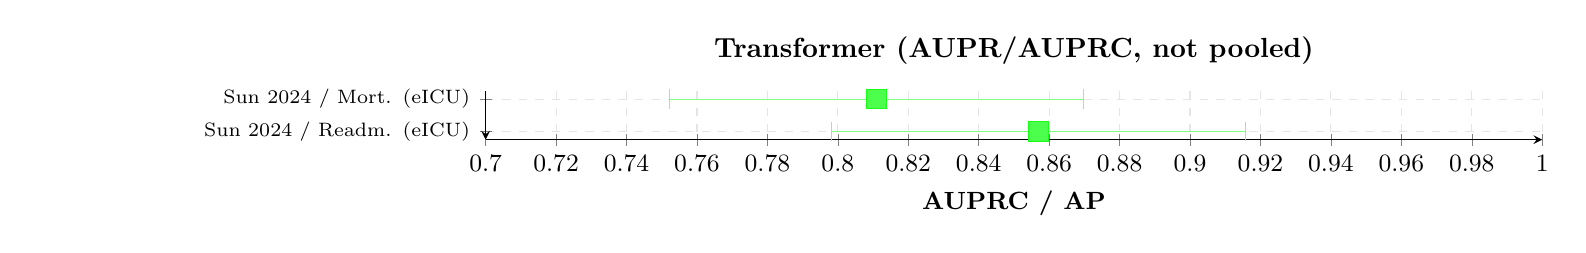
\begin{tikzpicture}[scale=1.0, every node/.style={scale=1.0}]
\begin{axis}[
    width=15cm, height=2.2cm,
    symbolic y coords={
        {Sun 2024 / Mort. (eICU)},
        {Sun 2024 / Readm. (eICU)}
    },
    ytick=data,
    y dir=reverse,
    xmin=0.70, xmax=1.00,
    xlabel={AUPRC / AP},
    xlabel style={font=\small\bfseries},
    yticklabel style={font=\scriptsize, text width=5.5cm, align=right},
    xticklabel style={font=\small},
    grid=major,
    grid style={dashed, gray!20},
    axis lines=left,
    clip=false,
    enlarge y limits=0.25,
    title={\textbf{Transformer (AUPR/AUPRC, not pooled)}},
    title style={font=\normalsize},
]

\addplot[only marks, mark=square*, fill=green!70, mark size=3.5pt, draw=green!90,
    error bars/.cd, x dir=both, x explicit, error bar style={thin, green!50}]
    coordinates {
(0.811,{Sun 2024 / Mort. (eICU)}) +- (0.0588,0)
(0.857,{Sun 2024 / Readm. (eICU)}) +- (0.0588,0)
    };

\end{axis}
\end{tikzpicture}
\caption{PR forest plot --- Transformer (AUPR/AUPRC). Both estimates are from Sun M. et al.~\cite{Sun2024}, the sole source for this model. Unlike this study's AUC-ROC
estimates, these are not excluded for quality reasons (AUC-PRC pooling does not
depend on the missing event counts) but are not pooled because no other study
reports AUC-PRC for Transformer ($k=1$ per outcome); shown per outcome rather than
mixed into one number (main text, Section~2.10.4). See main text Section~4.1 for
why these values should still not be compared at face value to the other studies'.}
\label{fig:fp_pr_transformer}
\end{figure}
\end{landscape}

\begin{landscape}
\subsection{Random Forest --- AUPR/AUPRC (2 entries, 1 study): not pooled}

\begin{figure}[H]
\centering
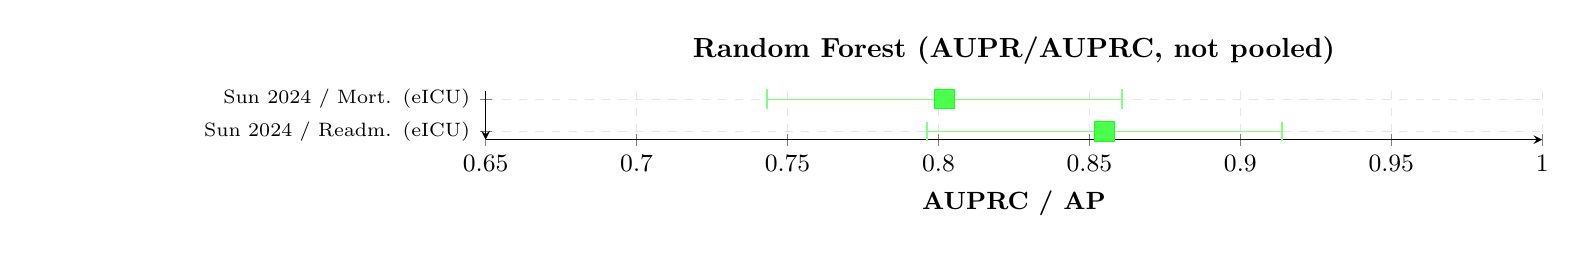
\begin{tikzpicture}[scale=1.0, every node/.style={scale=1.0}]
\begin{axis}[
    width=15cm, height=2.2cm,
    symbolic y coords={
        {Sun 2024 / Mort. (eICU)},
        {Sun 2024 / Readm. (eICU)}
    },
    ytick=data,
    y dir=reverse,
    xmin=0.65, xmax=1.00,
    xlabel={AUPRC / AP},
    xlabel style={font=\small\bfseries},
    yticklabel style={font=\scriptsize, text width=5.5cm, align=right},
    xticklabel style={font=\small},
    grid=major,
    grid style={dashed, gray!20},
    axis lines=left,
    clip=false,
    enlarge y limits=0.25,
    title={\textbf{Random Forest (AUPR/AUPRC, not pooled)}},
    title style={font=\normalsize},
]

\addplot[only marks, mark=square*, fill=green!70, mark size=3.5pt, draw=green!90,
    error bars/.cd, x dir=both, x explicit, error bar style={thin, green!50}]
    coordinates {
(0.802,{Sun 2024 / Mort. (eICU)}) +- (0.0588,0)
(0.855,{Sun 2024 / Readm. (eICU)}) +- (0.0588,0)
    };

\end{axis}
\end{tikzpicture}
\caption{PR forest plot --- Random Forest (AUPR/AUPRC). Both estimates are from Sun M. et al.~\cite{Sun2024}, the sole source for this model. Unlike this study's AUC-ROC
estimates, these are not excluded for quality reasons (AUC-PRC pooling does not
depend on the missing event counts) but are not pooled because no other study
reports AUC-PRC for RF ($k=1$ per outcome); shown per outcome rather than mixed
into one number (main text, Section~2.10.4). See main text Section~4.1 for why
these values should still not be compared at face value to the other studies'.}
\label{fig:fp_pr_rf_auprc}
\end{figure}
\end{landscape}

\newpage

\begin{landscape}
\subsection{Logistic Regression --- AUPR/AUPRC (2 entries, 1 study): not pooled}

\begin{figure}[H]
\centering
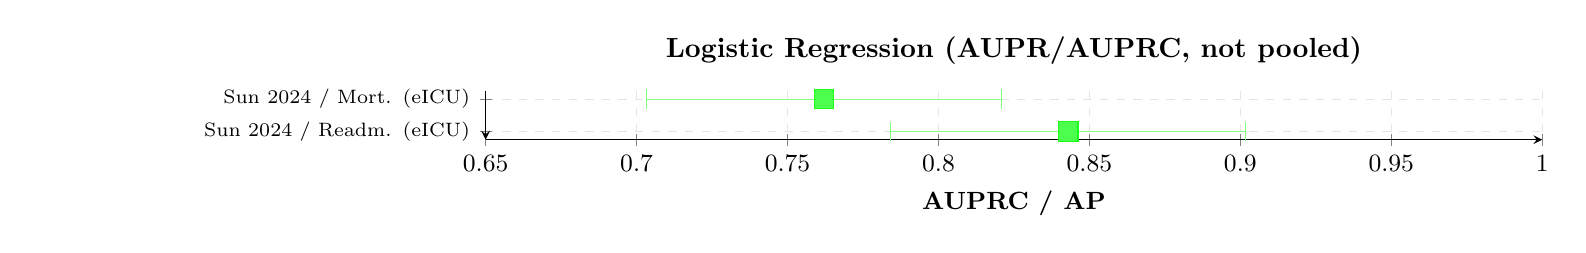
\begin{tikzpicture}[scale=1.0, every node/.style={scale=1.0}]
\begin{axis}[
    width=15cm, height=2.2cm,
    symbolic y coords={
        {Sun 2024 / Mort. (eICU)},
        {Sun 2024 / Readm. (eICU)}
    },
    ytick=data,
    y dir=reverse,
    xmin=0.65, xmax=1.00,
    xlabel={AUPRC / AP},
    xlabel style={font=\small\bfseries},
    yticklabel style={font=\scriptsize, text width=5.5cm, align=right},
    xticklabel style={font=\small},
    grid=major,
    grid style={dashed, gray!20},
    axis lines=left,
    clip=false,
    enlarge y limits=0.25,
    title={\textbf{Logistic Regression (AUPR/AUPRC, not pooled)}},
    title style={font=\normalsize},
]

\addplot[only marks, mark=square*, fill=green!70, mark size=3.5pt, draw=green!90,
    error bars/.cd, x dir=both, x explicit, error bar style={thin, green!50}]
    coordinates {
(0.762,{Sun 2024 / Mort. (eICU)}) +- (0.0588,0)
(0.843,{Sun 2024 / Readm. (eICU)}) +- (0.0588,0)
    };

\end{axis}
\end{tikzpicture}
\caption{PR forest plot --- Logistic Regression (AUPR/AUPRC). Both estimates are
from Sun M. et al.~\cite{Sun2024}, the sole source for this model. Unlike this
study's AUC-ROC estimates, these are not excluded for quality reasons (AUC-PRC
pooling does not depend on the missing event counts) but are not pooled because
no other study reports AUC-PRC for LR ($k=1$ per outcome); shown per outcome
rather than mixed into one number (main text, Section~2.10.4). See main text
Section~4.1 for why these values should still not be compared at face value to
the other studies'.}
\label{fig:fp_pr_lr_auprc}
\end{figure}
\end{landscape}

\begin{landscape}
\subsection{Random Forest --- AP (2 entries, 1 study)}

\begin{figure}[H]
\centering
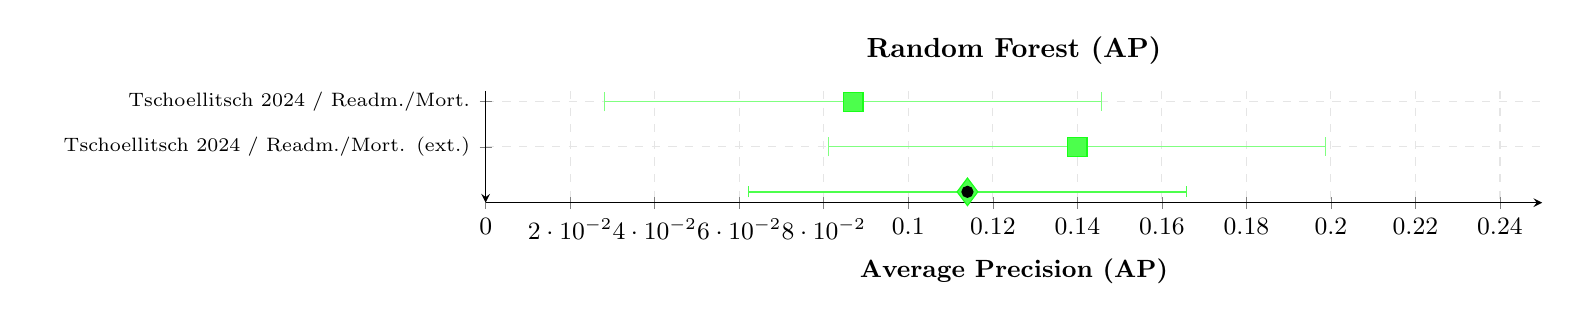
\begin{tikzpicture}[scale=1.0, every node/.style={scale=1.0}]
\begin{axis}[
    width=15cm, height=3.0cm,
    symbolic y coords={
        {Tschoellitsch 2024 / Readm./Mort.},
        {Tschoellitsch 2024 / Readm./Mort. (ext.)},
        Pooled effect
    },
    ytick=data,
    y dir=reverse,
    xmin=0.00, xmax=0.25,
    xlabel={Average Precision (AP)},
    xlabel style={font=\small\bfseries},
    yticklabel style={font=\scriptsize, text width=5.5cm, align=right},
    xticklabel style={font=\small},
    grid=major,
    grid style={dashed, gray!20},
    axis lines=left,
    clip=false,
    enlarge y limits=0.12,
    title={\textbf{Random Forest (AP)}},
    title style={font=\normalsize},
]

\addplot[only marks, mark=square*, fill=green!70, mark size=3.5pt, draw=green!90,
    error bars/.cd, x dir=both, x explicit, error bar style={thin, green!50}]
    coordinates {
(0.087,{Tschoellitsch 2024 / Readm./Mort.}) +- (0.0588,0)
(0.140,{Tschoellitsch 2024 / Readm./Mort. (ext.)}) +- (0.0588,0)
    };

\addplot[only marks, mark=diamond*, fill=green!70, mark size=5pt, draw=green!90]
    coordinates {(0.114,{Pooled effect})};
\addplot[only marks, mark=none, forget plot,
    error bars/.cd, x dir=both, x explicit, error bar style={thick, green!70}]
    coordinates {(0.114,{Pooled effect}) +- (0.0519,0)};

\end{axis}
\end{tikzpicture}
\caption{PR forest plot --- Random Forest (AP). Pooled effect: 0.114 (95\% CI: 0.062--0.165).}
\label{fig:fp_pr_rf_ap}
\end{figure}
\end{landscape}

\begin{landscape}
\subsection{XGBoost --- AP (2 entries, 1 study)}

\begin{figure}[H]
\centering
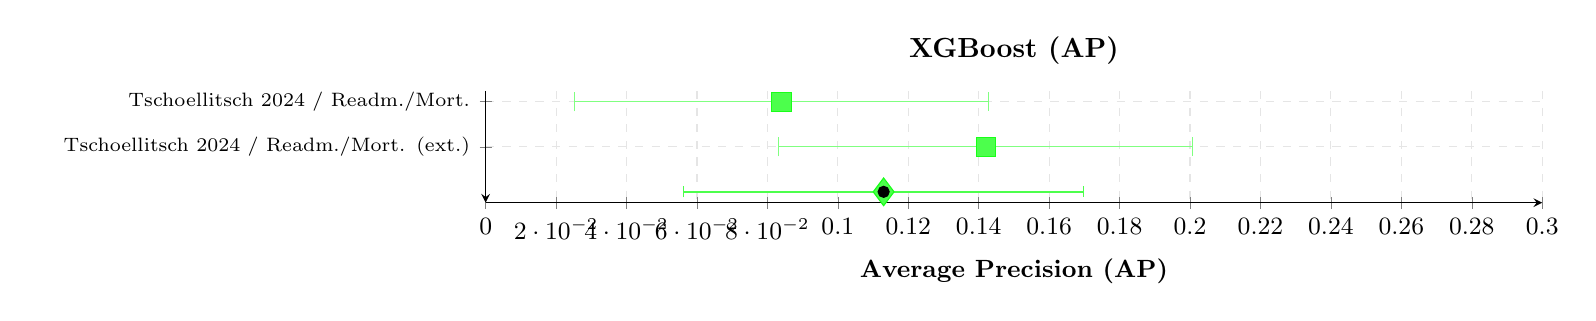
\begin{tikzpicture}[scale=1.0, every node/.style={scale=1.0}]
\begin{axis}[
    width=15cm, height=3.0cm,
    symbolic y coords={
        {Tschoellitsch 2024 / Readm./Mort.},
        {Tschoellitsch 2024 / Readm./Mort. (ext.)},
        Pooled effect
    },
    ytick=data,
    y dir=reverse,
    xmin=0.00, xmax=0.30,
    xlabel={Average Precision (AP)},
    xlabel style={font=\small\bfseries},
    yticklabel style={font=\scriptsize, text width=5.5cm, align=right},
    xticklabel style={font=\small},
    grid=major,
    grid style={dashed, gray!20},
    axis lines=left,
    clip=false,
    enlarge y limits=0.12,
    title={\textbf{XGBoost (AP)}},
    title style={font=\normalsize},
]

\addplot[only marks, mark=square*, fill=green!70, mark size=3.5pt, draw=green!90,
    error bars/.cd, x dir=both, x explicit, error bar style={thin, green!50}]
    coordinates {
(0.084,{Tschoellitsch 2024 / Readm./Mort.}) +- (0.0588,0)
(0.142,{Tschoellitsch 2024 / Readm./Mort. (ext.)}) +- (0.0588,0)
    };

\addplot[only marks, mark=diamond*, fill=green!70, mark size=5pt, draw=green!90]
    coordinates {(0.113,{Pooled effect})};
\addplot[only marks, mark=none, forget plot,
    error bars/.cd, x dir=both, x explicit, error bar style={thick, green!70}]
    coordinates {(0.113,{Pooled effect}) +- (0.0568,0)};

\end{axis}
\end{tikzpicture}
\caption{PR forest plot --- XGBoost (AP). Pooled effect: 0.113 (95\% CI: 0.056--0.170).}
\label{fig:fp_pr_xgboost_ap}
\end{figure}
\end{landscape}

\newpage

\begin{landscape}
\subsection{Ensemble --- AP (1 entry, 1 study)}

\begin{figure}[H]
\centering
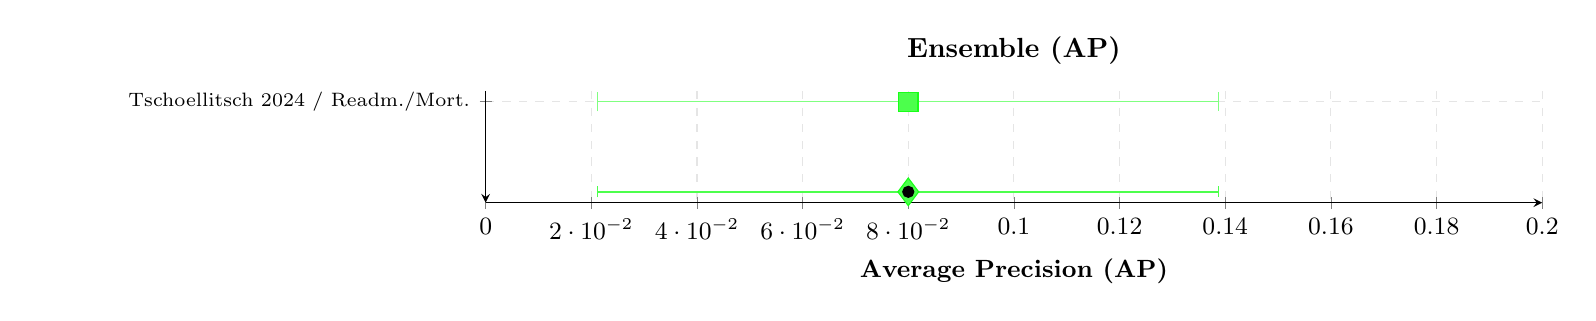
\begin{tikzpicture}[scale=1.0, every node/.style={scale=1.0}]
\begin{axis}[
    width=15cm, height=3.0cm,
    symbolic y coords={
        {Tschoellitsch 2024 / Readm./Mort.},
        Pooled effect
    },
    ytick=data,
    y dir=reverse,
    xmin=0.00, xmax=0.20,
    xlabel={Average Precision (AP)},
    xlabel style={font=\small\bfseries},
    yticklabel style={font=\scriptsize, text width=5.5cm, align=right},
    xticklabel style={font=\small},
    grid=major,
    grid style={dashed, gray!20},
    axis lines=left,
    clip=false,
    enlarge y limits=0.12,
    title={\textbf{Ensemble (AP)}},
    title style={font=\normalsize},
]

\addplot[only marks, mark=square*, fill=green!70, mark size=3.5pt, draw=green!90,
    error bars/.cd, x dir=both, x explicit, error bar style={thin, green!50}]
    coordinates {
(0.080,{Tschoellitsch 2024 / Readm./Mort.}) +- (0.0588,0)
    };

\addplot[only marks, mark=diamond*, fill=green!70, mark size=5pt, draw=green!90]
    coordinates {(0.080,{Pooled effect})};
\addplot[only marks, mark=none, forget plot,
    error bars/.cd, x dir=both, x explicit, error bar style={thick, green!70}]
    coordinates {(0.080,{Pooled effect}) +- (0.0588,0)};

\end{axis}
\end{tikzpicture}
\caption{PR forest plot --- Ensemble (AP). Pooled effect: 0.080 (95\% CI: 0.021--0.139).}
\label{fig:fp_pr_ensemble_ap}
\end{figure}
\end{landscape}

\begin{landscape}
\subsection{Logistic Regression --- AP (1 entry, 1 study)}

\begin{figure}[H]
\centering
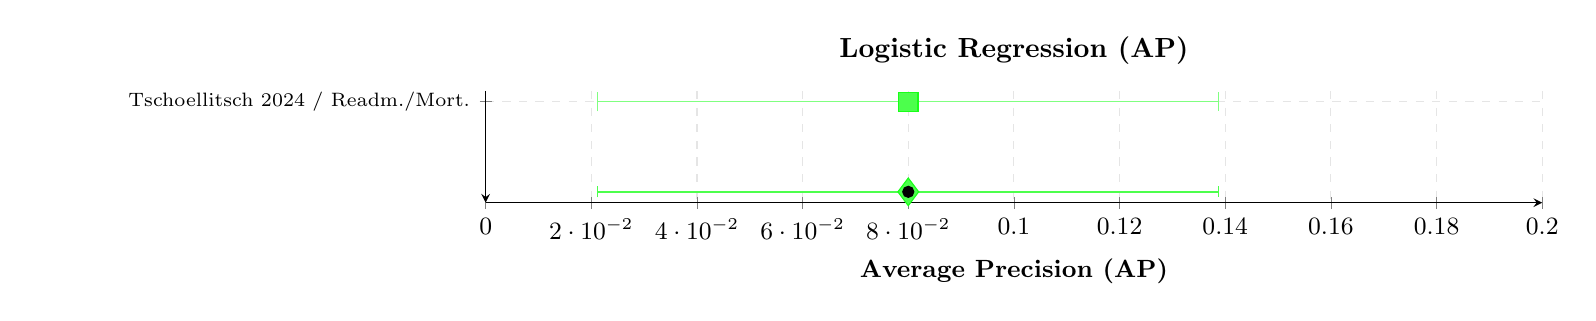
\begin{tikzpicture}[scale=1.0, every node/.style={scale=1.0}]
\begin{axis}[
    width=15cm, height=3.0cm,
    symbolic y coords={
        {Tschoellitsch 2024 / Readm./Mort.},
        Pooled effect
    },
    ytick=data,
    y dir=reverse,
    xmin=0.00, xmax=0.20,
    xlabel={Average Precision (AP)},
    xlabel style={font=\small\bfseries},
    yticklabel style={font=\scriptsize, text width=5.5cm, align=right},
    xticklabel style={font=\small},
    grid=major,
    grid style={dashed, gray!20},
    axis lines=left,
    clip=false,
    enlarge y limits=0.12,
    title={\textbf{Logistic Regression (AP)}},
    title style={font=\normalsize},
]

\addplot[only marks, mark=square*, fill=green!70, mark size=3.5pt, draw=green!90,
    error bars/.cd, x dir=both, x explicit, error bar style={thin, green!50}]
    coordinates {
(0.080,{Tschoellitsch 2024 / Readm./Mort.}) +- (0.0588,0)
    };

\addplot[only marks, mark=diamond*, fill=green!70, mark size=5pt, draw=green!90]
    coordinates {(0.080,{Pooled effect})};
\addplot[only marks, mark=none, forget plot,
    error bars/.cd, x dir=both, x explicit, error bar style={thick, green!70}]
    coordinates {(0.080,{Pooled effect}) +- (0.0588,0)};

\end{axis}
\end{tikzpicture}
\caption{PR forest plot --- Logistic Regression (AP). Pooled effect: 0.080 (95\% CI: 0.021--0.139).}
\label{fig:fp_pr_lr_ap}
\end{figure}
\end{landscape}

\begin{landscape}
\subsection{AdaBoost --- AP (1 entry, 1 study)}

\begin{figure}[H]
\centering
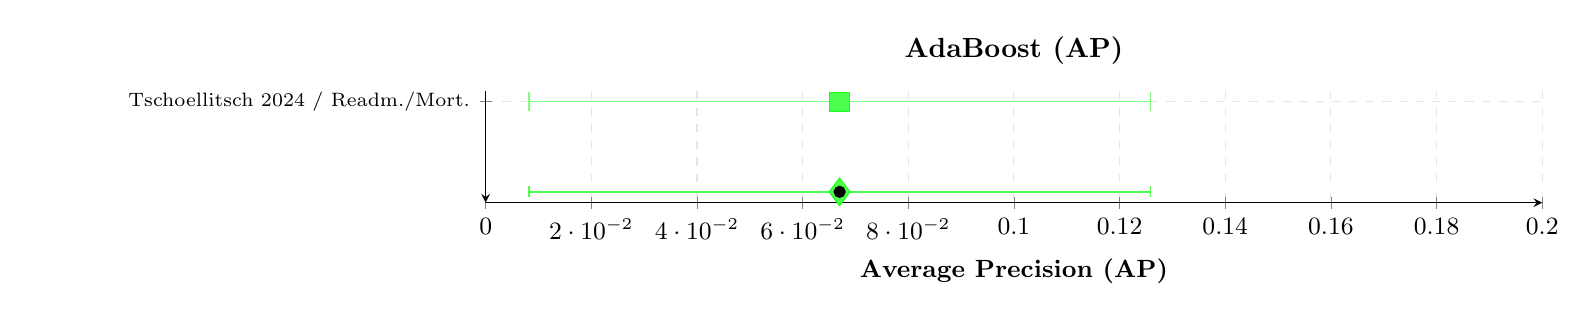
\begin{tikzpicture}[scale=1.0, every node/.style={scale=1.0}]
\begin{axis}[
    width=15cm, height=3.0cm,
    symbolic y coords={
        {Tschoellitsch 2024 / Readm./Mort.},
        Pooled effect
    },
    ytick=data,
    y dir=reverse,
    xmin=0.00, xmax=0.20,
    xlabel={Average Precision (AP)},
    xlabel style={font=\small\bfseries},
    yticklabel style={font=\scriptsize, text width=5.5cm, align=right},
    xticklabel style={font=\small},
    grid=major,
    grid style={dashed, gray!20},
    axis lines=left,
    clip=false,
    enlarge y limits=0.12,
    title={\textbf{AdaBoost (AP)}},
    title style={font=\normalsize},
]

\addplot[only marks, mark=square*, fill=green!70, mark size=3.5pt, draw=green!90,
    error bars/.cd, x dir=both, x explicit, error bar style={thin, green!50}]
    coordinates {
(0.067,{Tschoellitsch 2024 / Readm./Mort.}) +- (0.0588,0)
    };

\addplot[only marks, mark=diamond*, fill=green!70, mark size=5pt, draw=green!90]
    coordinates {(0.067,{Pooled effect})};
\addplot[only marks, mark=none, forget plot,
    error bars/.cd, x dir=both, x explicit, error bar style={thick, green!70}]
    coordinates {(0.067,{Pooled effect}) +- (0.0588,0)};

\end{axis}
\end{tikzpicture}
\caption{PR forest plot --- AdaBoost (AP). Pooled effect: 0.067 (95\% CI: 0.008--0.126).}
\label{fig:fp_pr_adaboost_ap}
\end{figure}
\end{landscape}

\begin{landscape}
\subsection{Neural Network --- AP (1 entry, 1 study)}

\begin{figure}[H]
\centering
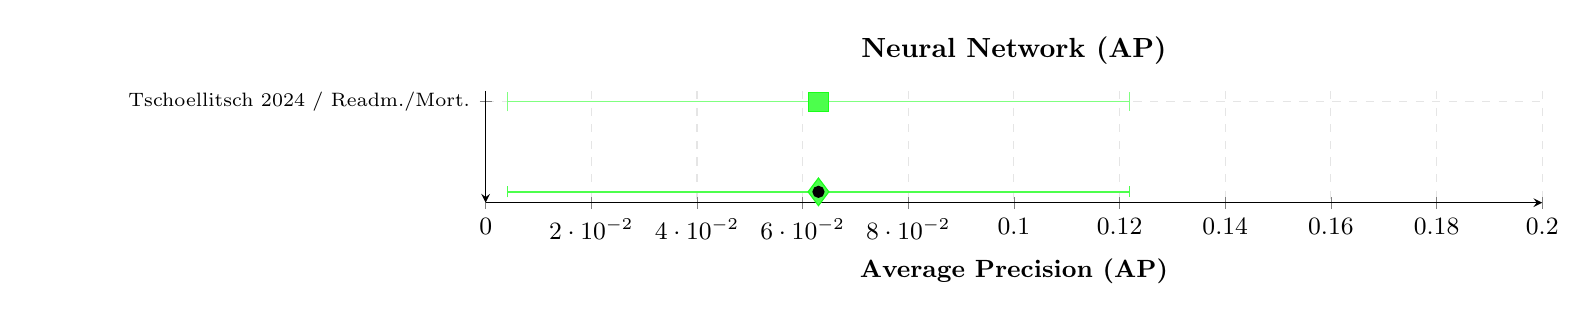
\begin{tikzpicture}[scale=1.0, every node/.style={scale=1.0}]
\begin{axis}[
    width=15cm, height=3.0cm,
    symbolic y coords={
        {Tschoellitsch 2024 / Readm./Mort.},
        Pooled effect
    },
    ytick=data,
    y dir=reverse,
    xmin=0.00, xmax=0.20,
    xlabel={Average Precision (AP)},
    xlabel style={font=\small\bfseries},
    yticklabel style={font=\scriptsize, text width=5.5cm, align=right},
    xticklabel style={font=\small},
    grid=major,
    grid style={dashed, gray!20},
    axis lines=left,
    clip=false,
    enlarge y limits=0.12,
    title={\textbf{Neural Network (AP)}},
    title style={font=\normalsize},
]

\addplot[only marks, mark=square*, fill=green!70, mark size=3.5pt, draw=green!90,
    error bars/.cd, x dir=both, x explicit, error bar style={thin, green!50}]
    coordinates {
(0.063,{Tschoellitsch 2024 / Readm./Mort.}) +- (0.0588,0)
    };

\addplot[only marks, mark=diamond*, fill=green!70, mark size=5pt, draw=green!90]
    coordinates {(0.063,{Pooled effect})};
\addplot[only marks, mark=none, forget plot,
    error bars/.cd, x dir=both, x explicit, error bar style={thick, green!70}]
    coordinates {(0.063,{Pooled effect}) +- (0.0588,0)};

\end{axis}
\end{tikzpicture}
\caption{PR forest plot --- Neural Network (AP). Pooled effect: 0.063 (95\% CI: 0.004--0.122).}
\label{fig:fp_pr_nn_ap}
\end{figure}
\end{landscape}


\section{Summary Tables}
\textit{See \texttt{results/tables/} for the full summary tables (AUC-ROC and PR detail and subgroup tables).}

\section{References}
\begin{enumerate}
\item Studies included in the PRISMA 2020 systematic review; see \texttt{references/references.bib}.
\end{enumerate}

\end{document}
